M%\documentclass[prd, nofootinbib, floatfix, 12pt]{revtex4}
%\documentclass[useAMS,usenatbib,11pt,preprint]{aastex}
%\documentclass[12pt,preprint]{aastex}
\documentclass[]{article}
\usepackage{amsmath}
\usepackage{amsbsy}
\usepackage{natbib}
\usepackage{graphicx}

\usepackage[paperwidth=8.5in,paperheight=11in,centering,hmargin=1in,vmargin=1in]{geometry}
%\usepackage[round]{natbib}
%\usepackage{float}
%\usepackage{amsmath}
%\usepackage{amsbsy}
\usepackage{caption}
\usepackage{subcaption}

\topmargin0.0cm
\textheight8.5in

%\input epsf
%\usepackage{amsmath,amssymb}
%\usepackage[margin=0in]{caption}
%\usepackage{subfigure}
%\usepackage{epsfig}
%\usepackage{color}
%\usepackage{ulem}
%\usepackage{epstopdf}

\renewcommand{\topfraction}{0.95}
\renewcommand{\bottomfraction}{0.95}


%%%%%%%%%%%%%%%%%%%%%%%%%%%%%%%%%%%%%%%%%%%%%%%%%%%%%%%%%%%%
%%%%%%%%%%%%%%%%%%%%%%%%%%%%%%%%%%%%%%%%%%%%%%%%%%%%%%%%%%%%
%%%%%%%%%%%%%%%%%%%%%%%%%%%%%%%%%%%%%%%%%%%%%%%%%%%%%%%%%%%%

\begin{document} 

\captionsetup{width=0.8\textwidth}

\title{The LSST Universe model and its validation}

\author{ Simon Krughoff, Andrew Connolly, Lynne Jones, Yusra AlSayyad,
  for the LSST Collaboration}

%\pagerange{\pageref{firstpage}--\pageref{lastpage}}

\label{firstpage}

\date{\today}

\maketitle 


\abstract{The Large Synoptic Survey Telescope (LSST) will produce a
  wide-field and multi-epoch imaging survey of 18,000 deg$^2$ of the
  southern sky.  The LSST has an 8.4m aperture (with an effective size
  of 6.7m) and a 9.6 deg$^{2}$ field of view.  The large etendue of
  the LSST enables the project to image the visible sky every 3
  nights. To evaluate the performance of the LSST, to design the
  algorithms used in processing the LSST data, and to enable the
  development of science analysis techniques in preparation for
  operations, the LSST has undertaken a program for high fidelity
  simulations.  These simulations include a realistic model of the
  universe (known as the base catalog or universe model), a framework
  for querying the model at specific points on the sky and instances
  in time (known as the catalog framework), and a fast ray-trace code for
  simulating raw images (PhoSim).  In this document we describe the
  base catalogs and catalogs framework (known together as CatSim) and
  validate them for use by the LSST project.  The requirements against
  which we will validate are described in the document ``Requirements
  for the LSST Simulation Framework''. }
 
\section{Introduction \label{sec:intro}}

A new generation of astronomical survey telescopes such as the Large
Synoptic Survey Telescope (LSST) will soon be surveying the universe
in unprecedented detail. Repeated observations of the same part of the
sky, with hundreds to thousands of observations over a period of ten
years, will enable detailed studies of the temporal universe (ranging
from transient sources such as supernovae and optical bursters, to
periodic variables such as Cepheids and RR-Lyrae stars, to moving
sources such as asteroids and high proper motion stars). Combination
of these observations will provide some of the deepest, large-scale
surveys of the universe ever undertaken and provide the ability to
measure the nature of dark energy with figures of merit 10-100 times
smaller than current surveys \citep[DETF][]{albrecht06}.

The stringent requirements on the statistical power of the LSST means
that we will soon no longer be limited by shot noise (i.e.\ the number
of sources within a sample) but by how well we can understand
systematic uncertainties within our data streams. These systematic
effects can arise from the design of the telescope (e.g.\ ghosting of
images or scatter light), from the response of the atmosphere (e.g.\
the stability of the point-spread-function or the variability in the
transmissivity of the sky), from the strategy used to survey the sky
(e.g.\ inhomogeneous sampling of astronomical light curves), or from
limitations in our analysis algorithms (e.g.\ due to the finite
processing power available approximations may need to be made when
characterizing the properties of detected sources). Understanding
which of these issues will impact the science from a given telescope
is critical if we hope to maximize their scientific returns.

Simulations of the data flow from survey telescopes can provide a
critical role in understanding the capabilities of an astronomical
system and in optimizing its scientific returns. By providing data
with the expected characteristics of a survey well in advance of first
light, algorithms and statistical techniques can be optimized and
scaled to the expected data volumes or new statistical approaches can
be developed to improve the data analysis.  In the following sections
we consider and describe how we model the astrophysical properties of
the universe that we expect the LSST to observe and validate the
properties of this model universe against the requirements of the
project \citep{requirements}.

\section{Source Catalogs and the Catalog Framework}

\subsection{Framework}

The design of a framework to simulate the data expected from the LSST
requires flexibility and scalability \citep{connolly10}.
%(to enable
%data generation runs that range from a single CCD image of a
%gravitational lens to images from thousands of full focal planes that
%trace the expected observing cadence of the survey). 
This is accomplished by dividing the simulation workload into three
separate components: a base component that stores a model of the
universe (including the distribution of galaxies from a cosmological
simulation, the distribution of stars from a Galactic Structure model,
and a model for the asteroid populations within our Solar System), a
system for querying the underlying model of the universe using
simulations of sequences of LSST observations, and a framework for the
generation of images via the ray-tracing of photons from individual
sources.

Figure~\ref{fig:flow} shows the flow of information through the LSST
simulation framework.
%Simulations of sequences of
%LSST observations enable catalogs of LSST sources to be
%generated. These catalogs can be analyzed for different science
%programs or passed to a photon based image generator that create input
%images for the data management analysis pipelines.  
This design enables the generation of a wide range of data products:
from all-sky catalogs used in modeling the LSST calibration pipeline,
to time domain data used to characterize variability as a function of
signal-to-noise and temporal sampling, to sequences of images of
gravitational lenses from which to measure cosmological time delays.
In this document we focus on the first component of the framework; the
LSST universe model or base catalog and how we can query this
model. This system is referred to as {\it CatSim} throughout this
document.

The base catalog is stored as a SQL database (using a Microsoft
SQLServer). Data are accessed through a Python interface that uses
SQLalchemy ({\tt http://www.sqlalchemy.org}) to provide a database
agnostic view of the sources. For LSST pointing, sources can be
queried as a function of position and time with the returned data
accounting for any change in brightness due to variability. For large
scale runs, the base catalog is queried using sequences of
observations derived from the Operations Simulator \citep{cook09} (see
also: {\tt http://www.lsst.org/lsst/opsim}).  The Operation Simulator
simulates LSST pointings that meet the cadence and depth requirements
of the LSST science cases while accounting for historical weather
patterns for Cerro Pachon and the visibility of the LSST footprint on
the sky. Each simulated pointing provides a position and time of the
observation together with the appropriate sky conditions (e.g. seeing,
moon phase and angle, and sky brightness). Positions of sources are
propagated to the time of observation (including the proper motion
information for stars and orbits for Solar System sources). Magnitudes
and source counts are derived using the atmospheric and filter
response functions appropriate for the airmass of the observation and
after applying corrections for source variability. The resulting
catalogs (instance catalogs) can be formatted for use in a science
application (e.g. measuring the proper motions of high velocity stars)
or fed to the final component of the simulation framework, the image
simulator \citep{phosim}.

The query framework is written in Python and takes an object-centric
view of the data.  For each object type (galaxy, main sequence star,
strong lens, etc.), a class is defined that knows how to query for,
format, and transform objects of that type.  Many objects are similar
in terms of their properties and how they need to be queried.  A small
number of base classes can, therefore, be defined that will encompass
the requirements of the majority of the object classes.  Additional
object types are then represented simply as subclasses of the base
class. Extensibility of catalog types is handled by a class called the
InstanceCatalog, which defines how the output from the object classes
is formatted and written out into a catalogs.  Again, each catalog
type is a subclass of the base InstanceCatalog class, so extending to
other catalog types simply requires overriding the default formatter.
This also allows for custom headers (like those needed for input to
PhoSim) and custom output (e.g. binary, fits, or Python pickle files).

Overall this approach provides a simple and extensible framework for
expressing different astrophysical sources and incorporating new
catalogs within an existing framework (i.e.\ different components of
the universe model are logically distinct and so can be separated into
independent tables in a database or in different databases all
together).

\begin{figure}[h]
\centerline{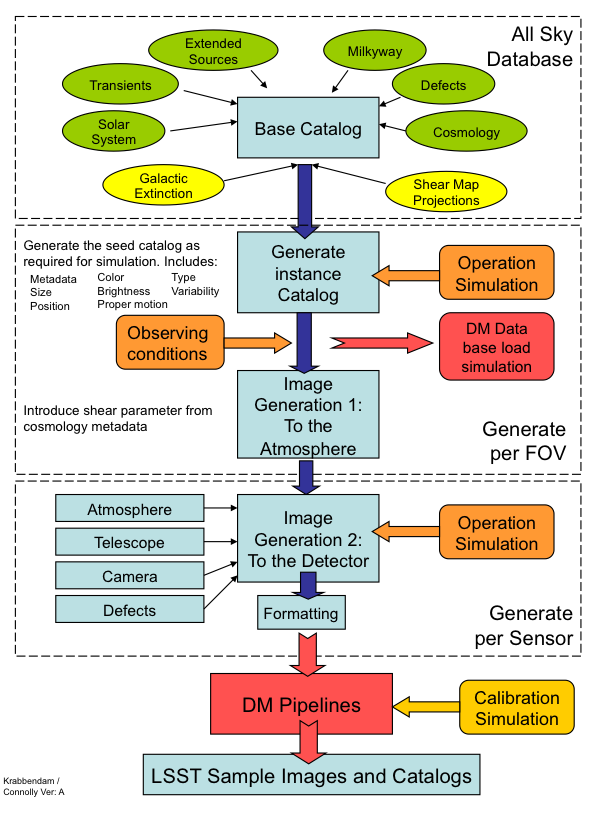
\includegraphics[width=0.5\textwidth]{validation_figures/flow.png}}
\caption{The flow of information through the LSST simulation
 framework. Databases of astrophysical sources are populated with
 models of the cosmological distributions of galaxies, the
 distributions of stars within our Galaxy, and the populations of
 asteroids within our Solar System. Using historical records for the
 weather at Cerro Pachon and the observing cadences required by the
 science drivers for the LSST, sequences of simulated observations
 are generated by the Operations simulator. From these simulated
 pointings, catalogs and images of galaxies can be generated that
 match the expected properties of the LSST system. Comparing the
 catalogs derived by processing the LSST data with those used to
 generate the inputs we enable a full end-to-end test of the LSST
 system.}
\label{fig:flow}       % Give a unique label
\end{figure}


\subsection{Galaxies and Cosmology \label{sec:gal}}

The galaxy simulation is based on dark matter haloes from the
Millennium simulation \citep{springel05} (with an assumed standard
$\Lambda$-CDM cosmology) and a semi-analytic baryon model grafted upon
the Millennium results as described in \citet{springel05} and
\citet{delucia}. This semi-analytic model features radiative cooling,
star formation, and the dynamics of black holes, supernovae, and
AGNs. It includes explicitly following dark matter haloes, even after
accretion onto larger systems, in order to follow the dynamics of
satellite galaxies for an extended period of time as well as 'radio
mode' feedback of AGNs. The model was adjusted to mimic the
luminosity, color, and morphology distributions of low redshift
galaxies \citep{delucia}. LSST cosmological catalogs were generated
from the \citet{delucia} data by constructing a lightcone, covering
redshifts 0$<$z$<$6, from 58 500h$^{-1}$Mpc simulation snapshots. This
lightcone covers a 4.5x4.5 degree footprint on the sky and samples
halo masses over the range $2.5\times10^9$ to $10^{12}$ $M_\odot$.

Dynamically tiling this footprint across the sky enables the
simulation of the full LSST footprint while keeping the underlying
data volume small (but at the expense of introducing periodicity in
the large scale structure).  For all sources, a spectral energy
distribution (SED), is fit to the galaxy colors using Bruzual and
Charlot spectral synthesis models \citep{bruzual}. The \citet{delucia}
catalog includes BVRIK magnitudes and dust values for the disk and
bulge components of each galaxy as well as radii, redshift,
coordinates, stellar age, masses and metallicities. These parameters
are used in constraining the assignment of SEDs to each disk and bulge
component.  Fits are undertaken independently for the bulge and disk
and include inclination dependent reddening. Morphologies are modeled
using two Sersi{\'c} profiles and a single point source (for the AGN)
with bulge-to-disk ratios and disk scale lengths from \citet{delucia}.
Half-light radii for bulges are estimated using the empirical
absolute-magnitude vs half-light radius relation given by
\citet{gonzalez09}.  AGNs are derived using the \citet{bongiorno12}
luminosity function. The B-band absolute magnitudes are converted to
bolometric luminosities using Eqn. 2 in \citet{hopkins07}. Empirical
relations derived from the SDSS enable computation of the colors and
stellar mass of the AGNs host galaxy from its luminosity. These
parameters are used, together with the redshift values from the AGN
catalog, to match each AGN to a galaxy in the galaxy catalog. In
general, the AGNs match to galaxies having higher stellar masses,
approximately $10^{9}$ to $10^{11}$ $M_{\odot}$ which is comparable to
recent analysis of host galaxies done by \citet{xue11}. The AGN SED is
taken from the mean AGN spectrum of \citet{vandenberk}.

Comparisons between the redshift and
number-magnitude distributions of the simulated catalogs with those
derived from deep imaging and spectroscopic surveys showed that the De
Lucia models under-predict the density of sources at faint magnitudes
and high redshifts. To correct for these effects, sources are
``cloned'' in magnitude and redshift space until their densities
reflect the average observed properties (see \S
\ref{sec:galaxycounts}).



\subsection{Galactic Structure \label{sec:stars}}

Stars are represented as point sources and are drawn from the Galfast model of \citep{galfast}.  
Galfast generates stars according to
density laws  derived from fitting SDSS data
to a thick and thin disk along with a halo \citep{juric}. Using an 
input luminosity function measured from SDSS for each class of star 
(main sequence, white dwarf, blue horizontal branch, etc.), Galfast samples stars in space and magnitude 
from a 4-dimensional probability density function
$\rho$(x,y,z,M). After this stage, using Fe/H and kinematics models
from \citet{ivezic08} and \citet{bond09} (also derived from SDSS data), 
each star is assigned a metallicity, proper motion, and parallax.
Spectral energy distributions are fit to the predicted
colors using the models of \citet{kuruczCD} for main sequence
stars and giants, \citet{bergeron95} for white dwarfs,
and a combination of spectral models and SDSS spectra for M, L, and T
dwarfs 
\citep[e.g.][]{cushing05,bochanski07,burrows06,pettersen89,kowalski10}. 
For Galactic reddening, a value of E(B-V) is assigned to each
star using the three-dimensional Galactic model of 
\citet{amores05}. For consistency with extragalactic observations the
dust model in the Milky Way is re-normalized to match the 
\citet{schlegel98} dust maps at a fiducial distance of 100 kpc.  Once the 
extinction and SED are assigned, observed magnitudes are calculated in
the SDSS and LSST photometric systems using fiducial system throughput curves.
Binary stars are included in the luminosity functions from which the
stellar colors are sampled but are assumed to be unresolved and
non-variable (except for a selection of eclipsing binaries described
later).

Stellar  populations included within the current implementation of the model are:
\begin{itemize}
\item Main Sequence: F,G,K,M,L,T
\item White Dwarf: H and He
\item Red Giant Branch
\item Blue Horizontal Branch
\item RR-lyrae
\item Cepheids
\end{itemize}

Approximately 10\% of the stellar sources are variable at a level detectable
by LSST.
Variability is modeled for sources within the base catalogs
by defining a light curve, its amplitude, a period, and a phase. For
queries that contain a time constraints the magnitude of the source is
adjusted based on the properties of the light curve (the current
implementation only allows for monochromatic variations in the
fluxes). Variables modeled range from cataclysmic variables, flaring
M-dwarfs, and micro-lensing events. For transient sources, the period
of the light curve is set to $>10$ years such that the sources will
not repeat within the period of the LSST observations.


\subsection{Solar System \label{sec:ssm}}

The Solar System model is a realization of the \citet{grav11} model.
All major groups of Solar System bodies are represented including:
main belt asteroids, near earth objects, trojans of the major planets,
trans-neptunian objects, and comets. There are approximately 11
million objects in the Solar System catalog with the vast majority (about 9 million) being
main belt asteroids. Populations are complete down to apparent
magnitudes of V=24.5.  Each object is assigned a carbonaceous or stony
composition spectrum derived from extending the reflectance spectra
from \citet{demeo} by linear extrapolation from 4500$\AA$ to 3000$\AA$
and then multiplying by a Kurucz solar spectrum. The choice of a
C or S type spectra for an object is assigned based upon a simple
relation to the size of its orbit that approximately matches SDSS
asteroid observations. Each object's brightness during a specific
observation is calculated from its location, phase, $H_V$ and g
values. $H_V$ is the object's absolute magnitude and corresponds to the
brightness if it were observed at 1 AU from the sun and at zero phase
angle.  The $H_V$ distribution is modeled independently for each
source population (NEO, TNO, main belt, etc.)  as described in \S 3 of
\citet{grav11}.  The g value relates the change in brightness of an
object with the change in phase and is set at 0.15 for all objects
across all bands, which is a typical value for asteroid phase curves.
A more accurate modeling of the asteroid phase curves would require
more realistic rotation and composition models which may be included
in future work.  The location of the Earth at the time of a
particular observation is incorporated through the orbital ephemeris software oorb
(\citet{granvik};{\tt http://code.google.com/p/oorb/}) that calculates a V
band apparent magnitude which is then used with the object's assigned
C or S type SED to derive the corresponding LSST band observations.

\subsection{Query Framework}




\section{Validation of the Simulation Framework Requirements}

In the following section we validate the current implementation of the
catalog simulation (CatSim) with respect to the LSST simulations
requirements (see \S 4.1 through \S 4.3 in
\citealt{requirements}). Following the structure in the requirements
document we consider the requirements on the properties of the
framework and then the properties of the underlying catalogs used for
the Universe model.  Where the current framework implementations do
not meet the requirements we discuss the impact of this and how we
will resolve this issue through future work.

\subsection{Framework: Requirement 1}

{\it  The simulation framework shall be open source and the input data, configurations,
and software shall be accessible by the LSST project and science
collaborations}\\

CatSim is released as open source software using the GPLv3 license
\citep{XXX}. The terms of this license are such that the software is
made available for copying, modification, and redistribution
(including derivative works). Adopting GPLv3 ensures that works
derived from the LSST software will also be released under the same
open-source licence. Code developed as part of CatSim (including
configuration files and example scripts) are stored in the LSST 
git repositories,

\begin{itemize}
\item {\tt https://dev.lsstcorp.org/cgit/LSST/sims/catalogs/generation.git/} -- Code to query
base catalogs.
\item {\tt https://dev.lsstcorp.org/cgit/LSST/sims/catalogs/measures.git/} -- Code to format
and manipulate catalogs produced by the generation packages.  This includes photometric, 
astrometric, and variability calculations.
\item {\tt https://dev.lsstcorp.org/cgit/LSST/sims/throughputs.git/} -- Repository
of system throughputs for the LSST reference design.
\end{itemize}

These repositories are available for anonymous (read-only) checkout or
(with a username and password) for read and write.

The source catalogs for the LSST Universe model are stored in a
Microsoft SQLServer database (SQLServer 2003) that is housed and
maintained at the University of Washington. All data stored within
this database are accessible using the CatSim framework and through
standard SQL queries.

\subsection{Framework Requirement 2}

{\it The simulation framework will be documented to a level
  that it can be installed and used by users external to the
  simulation team}\\

Documentation is available as web pages as well as self documenting
docstrings within the code.  This documentation includes installation
instructions, example applications, a description of the database
schema, and the interfaces and APIs used in CatSim. This documentation
is available at the following locations:
\begin{itemize}
\item catalog generation and measures -- {\tt http://www.astro.washington.edu/users/krughoff/documentation/}
\item base catalog schema and description -- {\tt https://dev.lsstcorp.org/trac/wiki/IS\_Catsim\_Database\_Documentation}
\end{itemize}


\subsection{Framework Requirement 3}

{\it  The interfaces between the components of the simulation framework shall be defined 
and documented}\\

The interfaces between the operations simulator (OpSim) and CatSim and
between CatSim and the photon simulator (PhoSim) are documented by the
OpSim and PhoSim teams respectively.  These interfaces are described in:
\begin{itemize}
\item OpSim to CatSim -- ({\tt https://lsstcorp.org/sites/default/files/SSTARUserGuide.pdf}; accessed 07/29/2013)
\item CatSim to PhoSim --{\bf XXX where is this}
\end{itemize}

\subsection{Framework Requirement 4} 

{\it The provenance within the data products shall be sufficient to rerun a simulation in a 
deterministic manner}\\

Provenance is maintain both internally to each component of a
simulator (e.g.\ for CatSim) as well as between each of the components
of the simulator framework through a series of mechanisms. For the
Operations Simulator each run of the simulator is given unique
identifier.  The OpSim identifier provides a unique table naming
convention in the OpSim database that is used by the CatSim query
framework to select the observing conditions given a pointing and an
OpSim run. 

For CatSim, the base catalog data is stored on disk and is
immutable. The base information going into any given run is therefore
the same.  Since the galaxies are tiled across the sky, the identifier
returned by the query framework is a combination of the tile number
and the identifier from the base catalog. This ensures that all
galaxies have a unique id and that that id is the same even if the
observational parameters (e.g. the bore site of the telescope) differ
from query to query.  The place where non-determinism may enter the
process is through the expression of the variability of the
astrophysical sources. Determinism for this process is ensured by
defining the initial time, $T_o$, for the light curve model (i.e.\
essentially specifying the phase of the light curve for a particular
time). A value for $T_o$ is assigned to all variable sources within
the catalog.  Stochastic variability, that uses a random number
generator (e.g.\ the damped random walk of an AGN light curve), have a
common seed for each source.
{\bf XXX is this true}

Special consideration must be paid to keeping ids in the output
catalogs unique.  Since each object database is independent (i.e.\
comprising a separate table or database), the ids will not be unique
when comparing one table to another. The tiling of the galaxy catalog
across the sky introduces a second method for introducing duplicates
in the catalog ids. To overcome these issues we apply a packing scheme
to ensure the original database id is recoverable from the catalog id.
Each object type is given an identifier that is unique across all
tables.  In practice, this is just an integer that is incremented when
a new table is added.  The unique id is then constructed by
bit-shifting the database id (or galtileid in the case of tiled
galaxies) and adding the object type id.  This assumes that there  will
not be more than 1024 object types.  
%The object type identifier is then added
%to the bit shifted id to create a new, unique id.

The input catalogs for the photon simulator includes a seed derived
from the visit id for a particular observation (i.e.\ obshistid from
the OpSim database). This seed is used to initialize the photon
simulator and for the photon generation. Since parallelism for the
photon simulator is on the chip level, the order of draws from the
random number generator for each chip is the same.


\subsection{Framework Requirement 5}

{\it The simulation framework shall be capable of running on individual workstations 
and high performance compute clusters}\\


CatSim runs naturally as a single core process since the problem is
parallelized on a pointing by pointing basis.  To parallelize CatSim
to larger systems many processes are run in a pleasingly parallel mode
with each process running a single pointing.  This approach marries
nicely with schedulers such as the Portable Batch System (e.g.\ {\tt
  http://www.pbsworks.com/}) and Condor \citep{condor}.  The
limitation on the level of parallelism is the database I/O.  The
current hardware (10 core, ??? GB, 40TB raid) has shown to be scalable
up to 70 concurrent processes, resulting in the generation of up to
~200 pointings or visits per day (this represents $\sim$20\% real time
data production).  The throughput of this system can be increase by
duplicating the database server or 
upgrading the hardware.

\section{Validation of the Requirements on the Catalog Simulations}

The simulation catalogs, in conjunction with tools for applying
astrometric and photometric operations and a framework for generating
observed catalogs, provide the requisite tools for conducting a
wide range of analysis activities. For example,
\begin{itemize}
\item the realized positions of solar system objects can be used to
  test moving object detection algorithms.
\item source catalogs can be used to test database and algorithm scaling.
\item inputs generated for PhoSim using the OpSim observing cadences
  enable large scale image simulations for sensitivity analyses and
  algorithm development.
\item realistic base catalogs enable the injection of specialized objects for specific science
analyses.
\item time domain catalogs of variable objects can be used in testing
  lightcurve recovery and characterization.
\end{itemize}

Each of the examples above requires a set of base catalogs that meet
the project needs.  Where extensions to the types and properties of
sources are required (e.g.\ by the LSST science community), support for
extensions of the query framework is required.

\subsection{Catalogs: Requirement 1}

{\it The LSST catalogs simulations shall contain representations of
  stars, galaxies, quasars, solar system objects, and variable sources
  with properties consistent with the LSST schema}\\

\subsubsection{Point, Extended and Moving Sources}

We have constructed a database to hold information about the sources
required by the Universal model.  Each of these source types has their
own schema (see sections \ref{sec:gal}, \ref{sec:stars}, and
\ref{sec:ssm} for galaxies, stars, and solar system sources
respectively).

The stellar database contains {\bf XXX} stars, covering the LSST
footprint (Dec $< +30^o$) with tables for main sequence and red giant
branch stars (??? stars), cepheids (), RR Lyrae (), blue horizontal
branch (), and white dwarfs ().  The stellar schema is describe in
{\tt http://ls.st/5jl}. For efficiency, large tables (e.g. the main
sequence stars) are stored in zones each of {\bf XXX} deg wide.  All
tables are indexed with a spherical tree built using a hierarchical
triangular mesh \citep[HTM][]{htm}.

Galaxies are stored in a single table $4.5^o \times 4.5^o$ on a side
with XXX galaxies. This single tile is then replicated across the sky
to provide the spatial coverage needed to simulate the survey (see
Figure \ref{fig:galcoverage}).  Tiling of the galaxies is handled in
the database using a stored procedure. % ({\tt  GalaxySearchSpecColsConstraint2013}).

The Solar System model is the most complicated table in the
database. The most general way to characterize Solar System objects is
through their orbital elements.  Propagating orbits to the time of
observation requires a numerical integration and, given the 11 million
sources in the Solar System model would be computationally prohibitive
for real-time calculation. We, therefore, pre-cache the postions of
asteroids within the database and interpolate their positions based on
the time of the observation.

Ephemerides are calculated for all Solar System sources within the
database for a ten year period. The time between ephemerides is
variable and depends on the asteroid population (i.e.\ it is set by
the velocity of the asteroid and the complexity of its orbital track).
{\bf XXX add the caching frequency from Yusra's email}. In total, {\bf
  XXX} object positions are stored within the Solar System table,
which, using a cubic {\bf XXX} interpolation, returns asteroid
positions with an accuracy of $<XXX$mas (sufficient to meet
requirement {\it Catalogs: Requirements 5}) These cached positions are
indexed using HTM \citep{XXX} to speed spatial lookup.

%, it is very slow with so many objects (11
%million total).  In order to keep query times reasonable the objects
%should be indexed so that it is fast to find objects that could
%possibly be within a particular aperture at a given time.  Ideally the
%index would identify exactly (to the precision required by LSST) the
%location of objects that land in the aperture are located at a given
%time.

For all sources, the generation of magnitudes and color, and the
application of time dependent astrometric corrections (e.g.
precession, parallax, proper motion) are calculated using Python
subclasses of the InstanceCatalog object.

\subsubsection{Variable Sources}
The framework is able to support several types of variability:
periodic, stochastic, and repeating.
The variability models used in the database include:.  
\begin{itemize}
\item M-dwarf flares -- full sky
\item AGN/QSOs -- full sky
\item RRly -- full sky
\item Cepheids -- exemplar individuals
\item Eclipsing binaries -- exemplar individuals
\item Am CVn -- exemplar individuals
\item Micro lensing -- exemplar individuals
\end{itemize}
Each type of variability is described by either a parametric model or
an interpolated lookup table.  To date only mono-chromatic variability
has been implemented (see Figure \ref{fig:lcs} for example lightcurves).

Variable sources are implemented through the InstanceCatalog API
\citep{XXX}. This API takes the name of the variability model and the
parameters associated with that model (both of which are stored in the
database) and modifies the brightness of a source based on the time of
observation.

\subsection{Catalogs: Requirement 2}

{\it At high Galactic latitudes the average number densities of
  sources shall be within 20\% and 10\% of the observed counts for
  stars and galaxies and galaxies respectively (to the $5\sigma$ point
  source coadded depth of LSST)} \\

%Stellar number densities at Galactic latitudes closer than to the
%plane than $|b| < 30^o$ are difficult to model due to the rising
%density and resulting confusion and deblending issues.  For these
%reasons, the criterion for stellar number counts at low latitudes are
%relaxed to $\pm 30\%$.  For stars where $|b| > 30^o$, the Galfast
%model has been vetted against the SDSS data.  For stars with $|b| <
%30^o$, we quantify the uncertainty in the model by comparing two
%reference models for Galactic structure.  We compare the realization
%of the Galfast model to a realization of the \citet{besancon} model.

\subsubsection{Stars}
We take six representative fields at varying Galactic latitudes and at
two longitudinal values (one toward the bulge, $b=0$, and one directly
away, $b=180$).  We compare number counts of main sequence stars to
the co-added limiting magnitude in the i-band from the Galfast model
\citep{XXX} using the composite dust model of \citet{amores05}
normalized to \citet{schlegel98} to the \citet{besancon} model with
their dust model.  Figure \ref{fig:scounts_0} shows the cumulative
number counts as a function of magnitude for the Besan\c{c}on (dashed)
and Galfast (solid) models for six values of galactic longitude toward
the galactic bulge.  We are interested in the fractional cumulative
contribution.  In Figure \ref{fig:sratio_0} we plot the ratio of
Besan\c{c}on counts to Galfast counts for the six test fields shown in
Figure \ref{fig:sratio_0}.  The dashed lines are the $\pm30\%$ limits
for the low latitude sizing model constraints and the dash-dot lines
are the $\pm18\%$ limits for the high latitude limits.  Since the
number counts are dominated by the faint end, it's most important
where the lines end up at faint magnitudes for sizing considerations
(the co-added depth for the i-band is 26.8).  Nominal single epoch
depth for i-band is 24.0.

In the case directed toward the galactic bulge, all fields meet the
requirements at the co-added depth except for $b=-10$.  At the nominal
single epoch depth, the $b=-10$ case fails and the $b=-30$ case misses
the $\pm18\%$ requirement, but makes the $\pm30\%$ requirement.

For the high latitude fields away from the galactic bulge, the
deviation from the Besan\c{c}on model is within the stated
requirement.  The $b=-10$ case, the number counts from Galfast
significantly under predict relative to the Besan\c{c}on model.  The
$b=-30$ case shows similar, though not as drastic, under prediction
and misses the requirement for all but the faintest magnitudes and
even then only meats the $\pm30\%$ requirement.

%We repeated this analysis using the GALFAST dust model and the results do not change significantly


\begin{figure}[h]
\centering
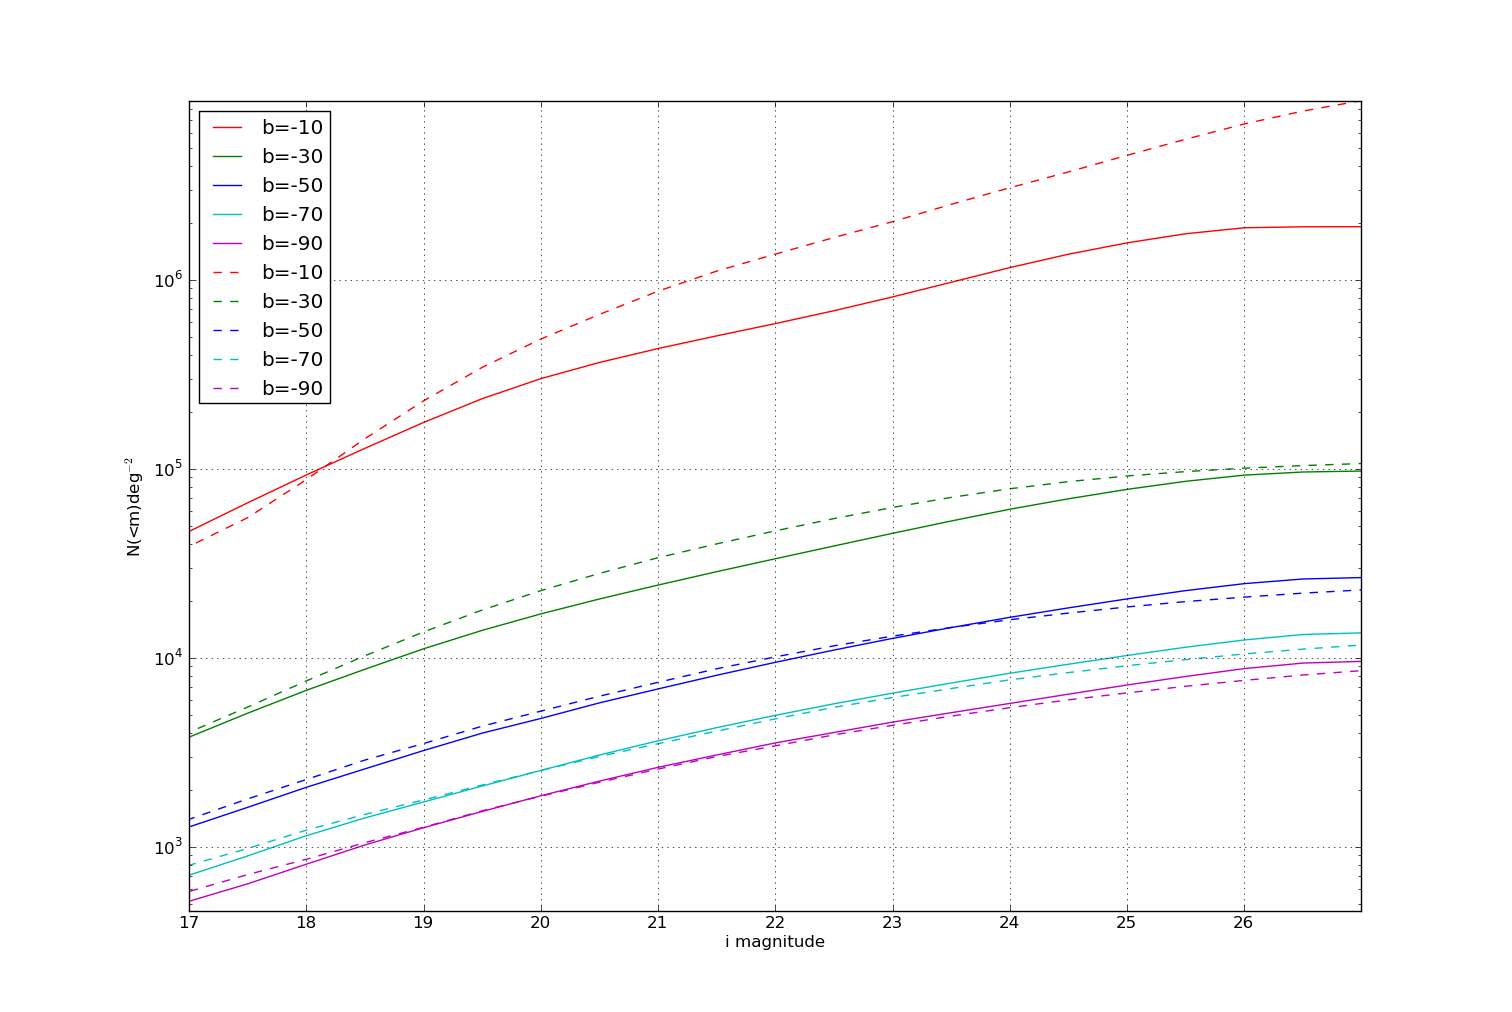
\includegraphics[width=5in]{validation_figures/cumulative_stars_0_besancon_dust.png}
\caption{Cumulative counts of stars from the Besan\c{c}on (dashed) and Galfast (solid) models for 5 representative fields toward the Galactic bulge (l=0$^o$) \label{fig:scounts_0}}
\end{figure}

\begin{figure}[h]
\centering
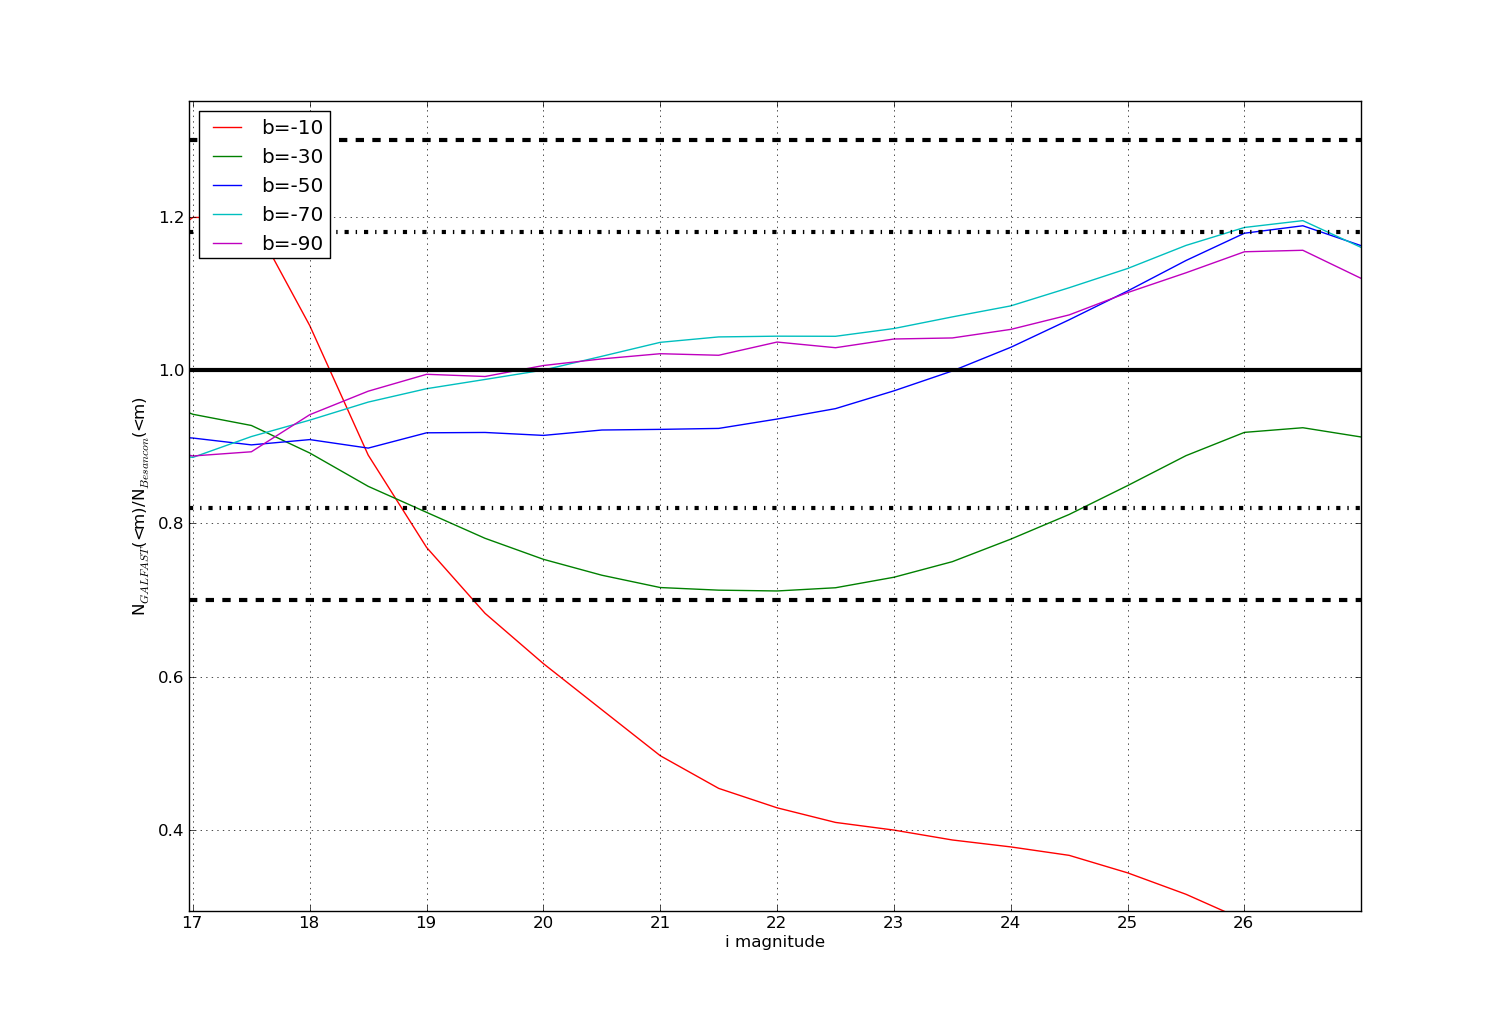
\includegraphics[width=5in]{validation_figures/cumulative_ratio_stars_0_besancon_dust.png}
\caption{Cumulative ratio of counts of stars from the Besan\c{c}on and Galfast models for 5 representative fields toward the Galactic bulge (l=0$^o$) \label{fig:sratio_0}}
\end{figure}

\begin{figure}[h]
\centering
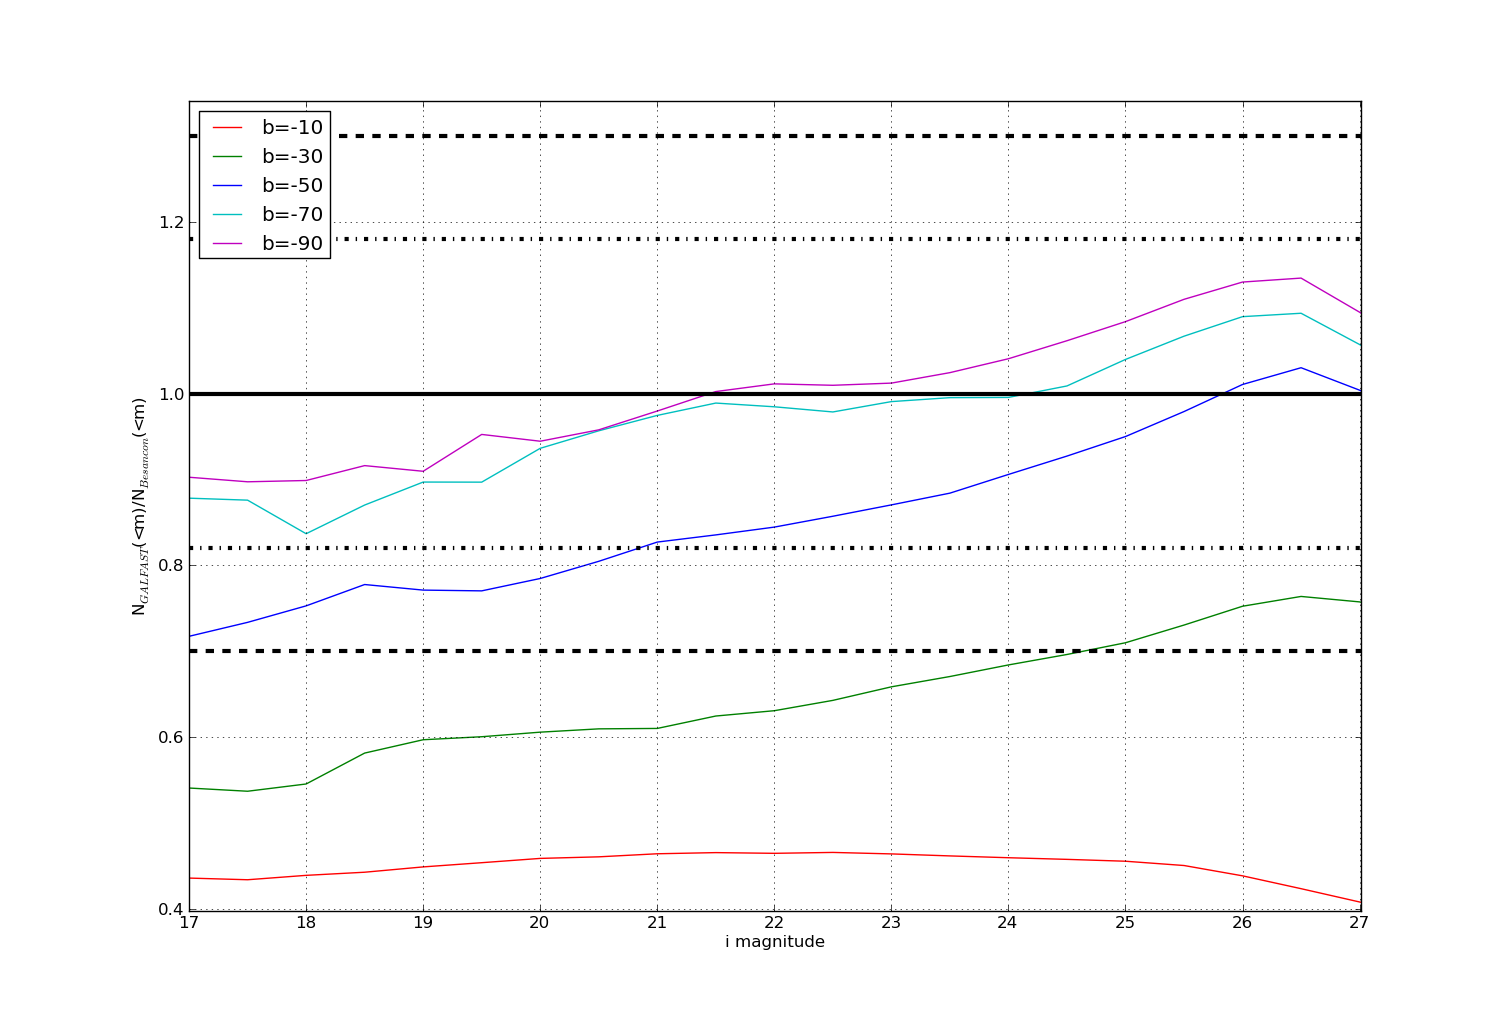
\includegraphics[width=5in]{validation_figures/cumulative_ratio_stars_180_besancon_dust.png}
\caption{Cumulative ratio of counts of stars from the Besan\c{c}on and Galfast models for 5 representative fields away from the Galactic bulge (l=180$^o$) \label{fig:sratio_180}}
\end{figure}

\subsubsection{Galaxies \label{sec:galaxycounts}}

Figure \ref{fig:gcounts} shows a comparison of the galaxy counts in
CatSim to observations provided by Metcalfe et al. (see {\tt
  http://star-www.dur.ac.uk/~nm/pubhtml/counts/counts.html}).  This
comparison is undertaken in the $i$ band to minimize the effects of
dust extinction which are somewhat uncertain in the Durham
compilations.  A single transform of I$_{kc}$ = i$_{AB}$ - 0.5 is
applied to the Metcalfe magnitudes to take them from the Kron-Cousins
photometric system to AB photometric system. For magnitudes $i<25.5$
the simulated number counts are consistent with the compilation of
galaxy counts. For magnitudes fainter than $i=25.5$ the simulated
number counts are systematically lower that the observations.

In Figure \ref{fig:gratio} illustrate this further by plotting the
ratio of the cumulative counts taken from the simulations to a
polynomial fit to the cumulative counts derived from the Metcalfe
data.  The error bars are estimated from the published uncertainties
on the Metcalfe number counts. The requirement on the galaxy densities
is that it is within $\pm10\%$ of the observed counts (to a coadded
i-band depth of 26.8). This requirement is set from the variance in
the observed counts due to the small size of galaxy surveys at the
limit of the LSST data.
% We have
%taken their compilations from: {\tt
%  http://star-www.dur.ac.uk/~nm/pubhtml/counts/idata.txt} accessed on
%06/01/2013. 

\begin{figure}[h]
\centering
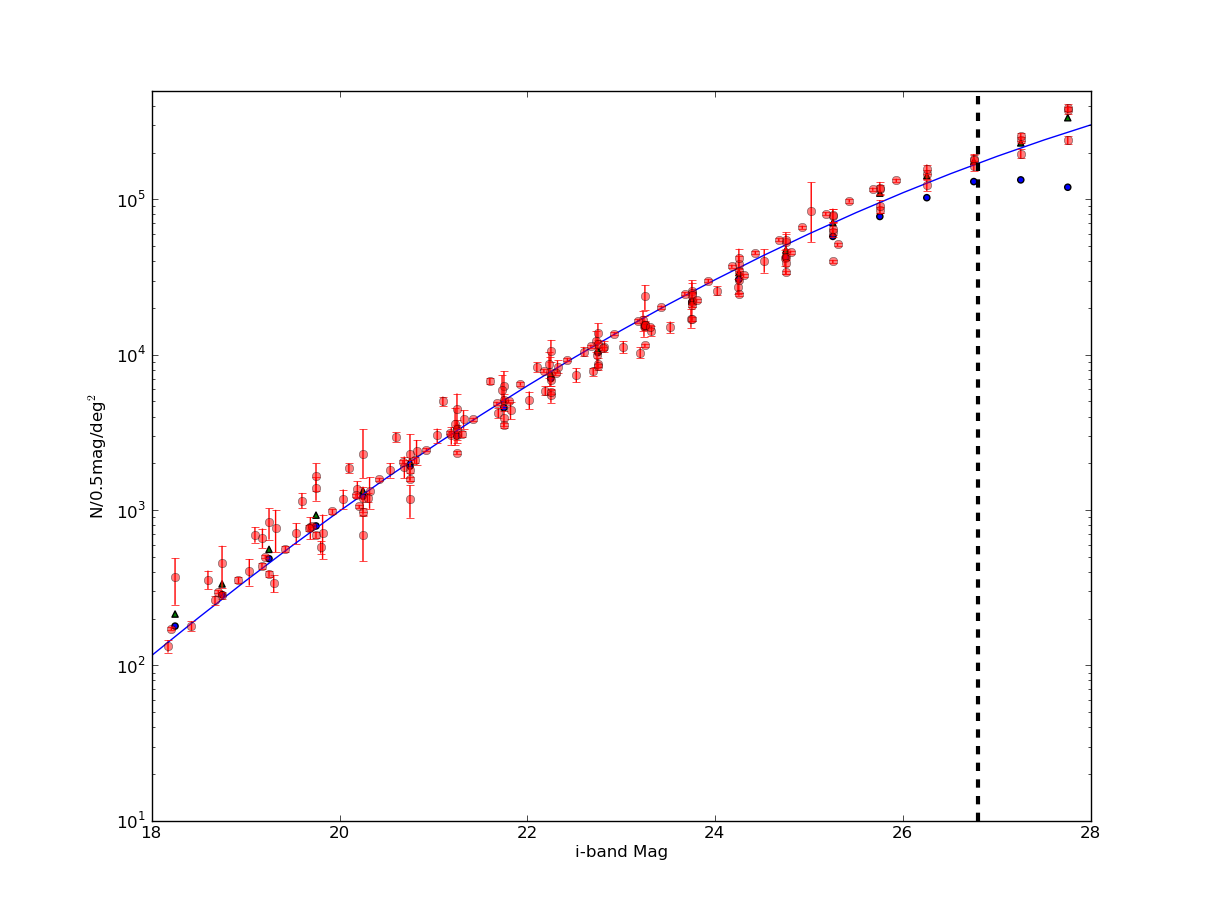
\includegraphics[width=0.45\textwidth]{validation_figures/Ngals-i.png}
\hfil 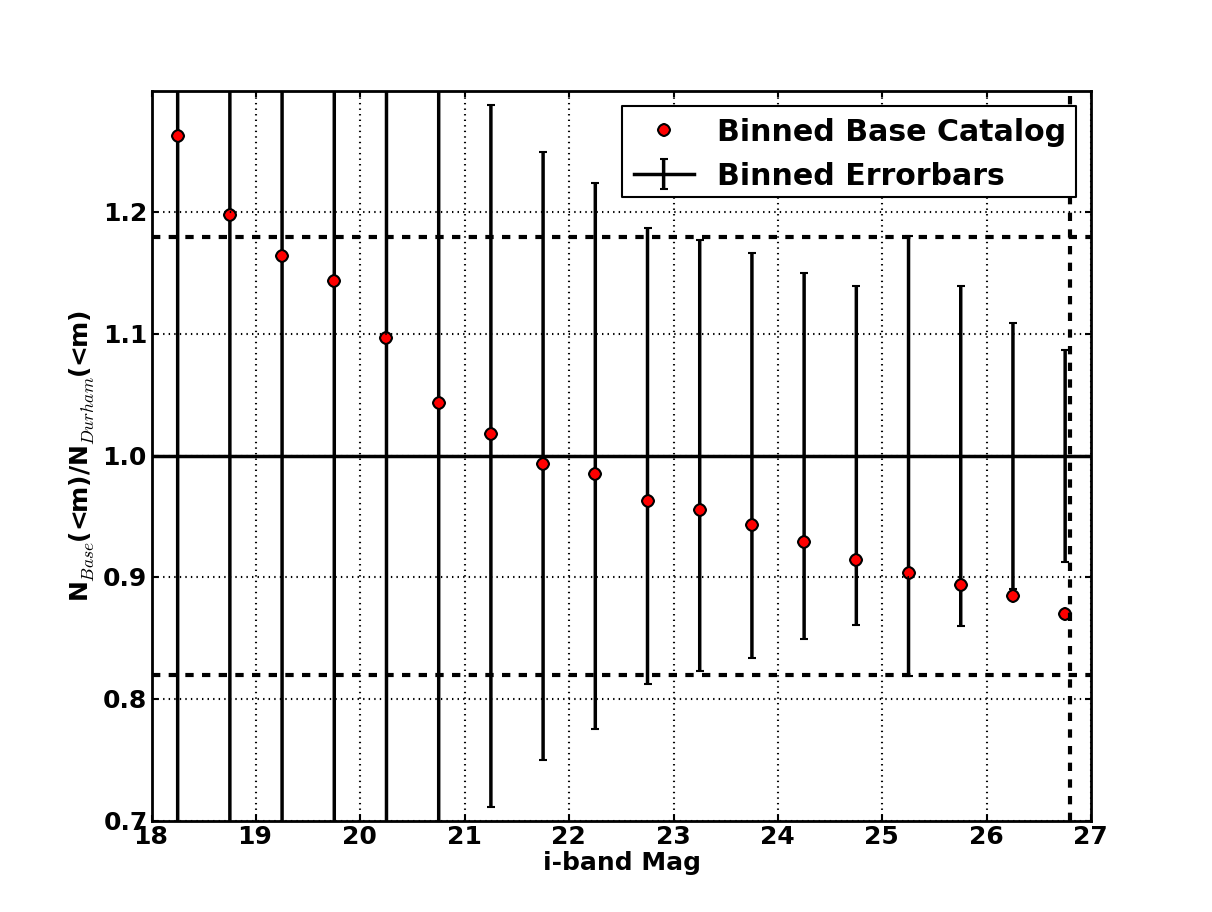
\includegraphics[width=0.45\textwidth]{validation_figures/CumulativeFraction_i.png}
\caption{A comparison of the Metcalfe galaxy number counts (symbols)
  to those derived from the simulated catalog \label{fig:gcounts}. The
  left panel shows the differential counts and the right panel the
  ratio of the cumulative counts. Error bars are from derived from
  those published by the individual surveys. \label{fig:gratio}
The vertical dashed line represents the
  5$\sigma$ magnitude limit for galaxies.}
\end{figure}

\subsubsection{Ramifications of missing requirements}


{\bf XXX Redo}
At low galactic latitudes the models for the stars are uncertain at a
level greater than the requirements (i.e the discrepancy between
Galfast and Besan\c{c}on is > {\bf XX}\%).  This has the potential to
impact the sizing and compute models for the LSST.

The validity of the Besan\c{c}on as ground truth in the plane of the
galaxy is not obvious.  In fact, SDSS and Galfast star counts agree
surprisingly well at low galactic latitudes (private communication
with M. Juri\'{c}).  However, the completeness of SDSS deep in the
plane has also not been quantified.  Certainly in the densest regions
of the plane there is significant loss of stars due to blending.
Further, since the Besan\c{c}on models are drawn from distributions
with binary corrections applied and the Galfast model does not produce
unresolved binary systems as multiple objects in the catalogs, the
Galfast models will under-predict relative to the Besan\c{c}on by
approximately the unresolved binary fraction.  These questions will be
resolved through an ongoing comparison to observations from other
surveys (e.g. Pan-STARRS).

\subsection{Catalogs:  Requirement 3}

{\it Size, ellipticity, and redshift distributions of galaxies shall
  be representative of those observed by extant space and ground-based
  telescopes and, for a fiducial image quality of 0.72 arcsec,
  deviations from the observed distributions shall contribute $<20$\%
  of the observed effective density of galaxies, n$_{eff}$, used in
  the weak lensing samples (assuming a fiducial value of n$_{eff} =
  28$ galaxies per arcmin$^2$)}\\


The ability to use gravitational weak lensing to constrain
cosmological parameters is dependent on $n_{eff}$, the effective
density of galaxies on the sky that can be used in weak lensing
measurements. The size of $n_{eff}$ depends on the inherent shape
noise of the galaxies, the size distributions of the galaxies relative
to the size of the PSF, and the signal-to-noise of the observations.
Following the methodology of \citet{chang} we calculate $n_{eff}$ for
the distributions in the base galaxy catalog.  In summary, we use
Equation 9 to calculate $n_{eff}$:
\begin{equation}
n_{eff} = \frac{1}{\Omega}\sum^N_i\frac{\sigma^2_{SN}}{\sigma^2_{SN}+\sigma^2_{m,i}}
\end{equation}
where $\sigma_{SN}$ is the intrinsic shape noise, $\sigma_{m,i}$ is
the shape measurement noise for the i$^{th}$ galaxy, and $N$ is the
number of galaxies in the sample. The shape noise is derived from the
ellipticity distribution of the galaxies, with $\sigma_{SN} = 0.26$
\citep{chang}.  The measurement noise can be approximated using
Equation 13 of \citet{chang}:
\begin{equation}
\sigma_m(\nu,R) = \frac{a}{\nu}\left[1+\left(\frac{b}{R}\right)^c\right]
\end{equation}
where $\nu$ is the signal-to-noise ratio of the source,
$R=\frac{r_{gal}^2}{r_{PSF}^2}$ is the area of the galaxy relative to
the point spread function.  We adopt values from \citet{chang} of
(a,b,c) = (1.58,5.03,0.39), and assume a fiducial PSF size of 0.7
arcsec. We use an estimate for the limiting magnitude of the co-added
images of 26.7.  {\bf XXX why?} This takes into account the fact that
the measurements are on extended sources as well as the fact that the
SRD value of 27.5 in r is for dark sky observations at zenith.  The
galaxy sample is the ``Gold Sample'' of galaxies with $i < 25.3$.  For
each galaxy, $r_{gal}$ can be calculate from the flux ratio of the
bulge and disk components as well as the effective half light radii of
each component (see Appendix B in \citet{chang} for a derivation of
this calculation).

Using this framework, we test the sensitivity of the measured
$n_{eff}$ on our assumptions for the ellipticity, size, magnitude, and
redshift distributions of the galaxies in the Universe model.  For all
calculations that follow we use the k=1 criterion of \citet{chang}
meaning that galaxies with $\sigma_m < \sigma_{SN}$ are culled from
the sample. This assumes that no improvement has been made in the
measurement of shear over current techniques.  The galaxy shape noise
distribution has been measured by the COSMOS project \citep{cosmos}
and, to first order, the dependence of $n_{eff}$ on the shape of the
distribution can be expressed in terms of the variance of the
ellipticity distribution. The dependence of $n_{eff}$ on apparent
magnitude arises due to the steepness of the galaxy number counts. As
is shown in Figure \ref{fig:neffvm}, however, due to the decrease in
signal-to-noise of the sources there is a sharp cut-off in the value
of $n_{eff}$ at $i=24.5$.  Given this, galaxy redshift distributions
must agree with observations to a limiting magnitude of $i=24.5$ to
insure an accurate mapping between physical and angular size.
Finally, the size distribution of the combined two component galaxy
model must reproduce the measured distributions.

The ellipticity distribution is measured from the base catalog by
sampling the composite Sersi{\'c} (bulge and disk together) using the
ellipsoid parameters and the appropriate flux ratio for each galaxy.
The moments are measured and ellipticities calculated using the
definitions in \citet{chang}.
\begin{equation}
\epsilon_1 = \frac{I_{11}-I_{22}}{I_{11}+I_{22}+2\sqrt{I_{11}I_{22} - I^{2}_{12}}}\\
\epsilon_2 = \frac{2I_{12}}{I_{11}+I_{22}+2\sqrt{I_{11}I_{22} - I^{2}_{12}}}
\end{equation}
where $\epsilon_1$ and $\epsilon_2$ are the $x$ and $y$ components of
the ellipticity and $I_{11}$, $I_{12}$, $I_{22}$ are the variance and
covariance of the moments of the light distribution.

The measured variance in the ellipticity distribution of the galaxies
in the simulation catalog is $\sigma_{SN} = 0.26$; identical to that
reported by \citet{chang}. The shape differs slightly from the COSMOS
distribution with a broader tail and wider central component. (see
Figure \ref{fig:ellip1} and Figure \ref{fig:ellip2}).  As shown in
Figures~\ref{fig:ellip_errsmall} and \ref{fig:ellip_errbig} these
slight variations in ellipticity distribution will not impact the
measured value of $n_{eff}$ (Figures \ref{fig:ellip_errbig} and
\ref{fig:ellip_errsmall} show the ellipticity distributions of samples
of galaxies that will fail to meet the requirements on $n_{eff}$).

\begin{figure}[H]
\centering
\begin{subfigure}[b]{0.3\textwidth}
               \centering
              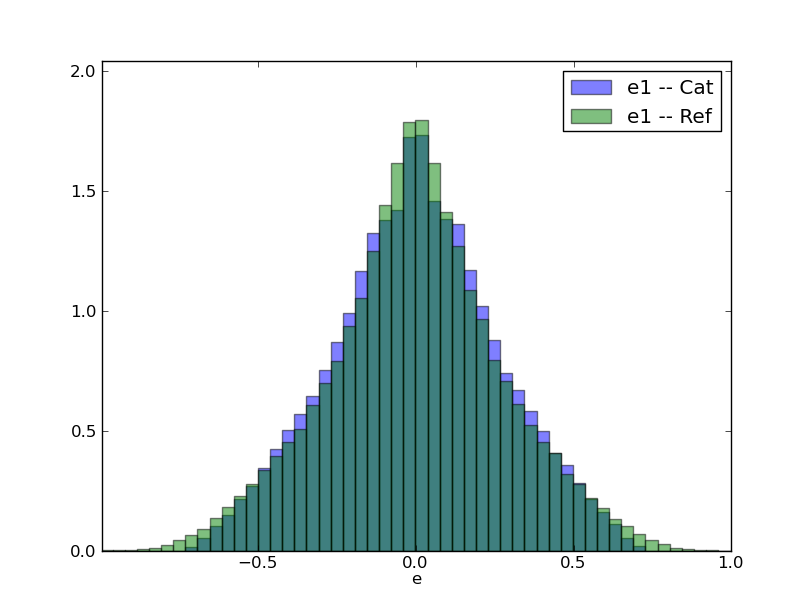
\includegraphics[width=\textwidth]{validation_figures/e1_hist.png}
               \label{fig:ellip1}
        \end{subfigure}
        \begin{subfigure}[b]{0.3\textwidth}
               \centering
               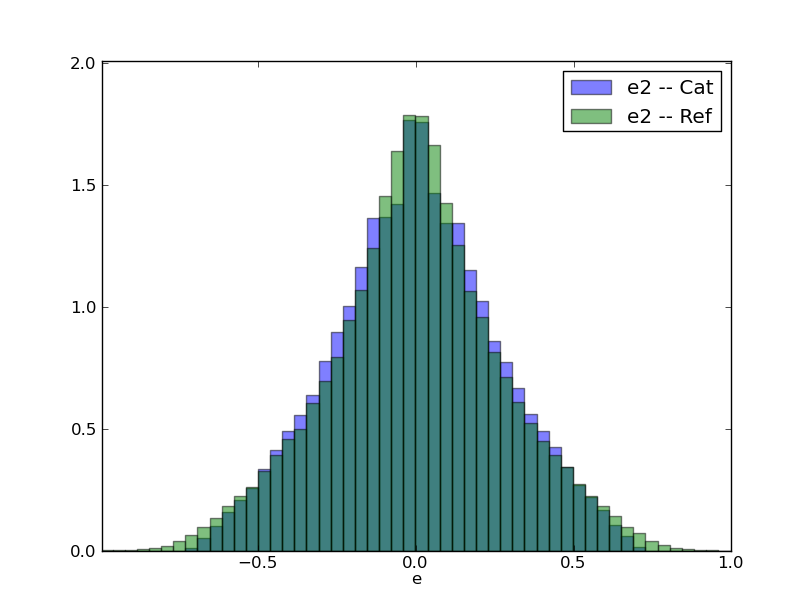
\includegraphics[width=\textwidth]{validation_figures/e2_hist.png}
               \label{fig:ellip2}
      \end{subfigure}

        \begin{subfigure}[b]{0.3\textwidth}
              \centering
              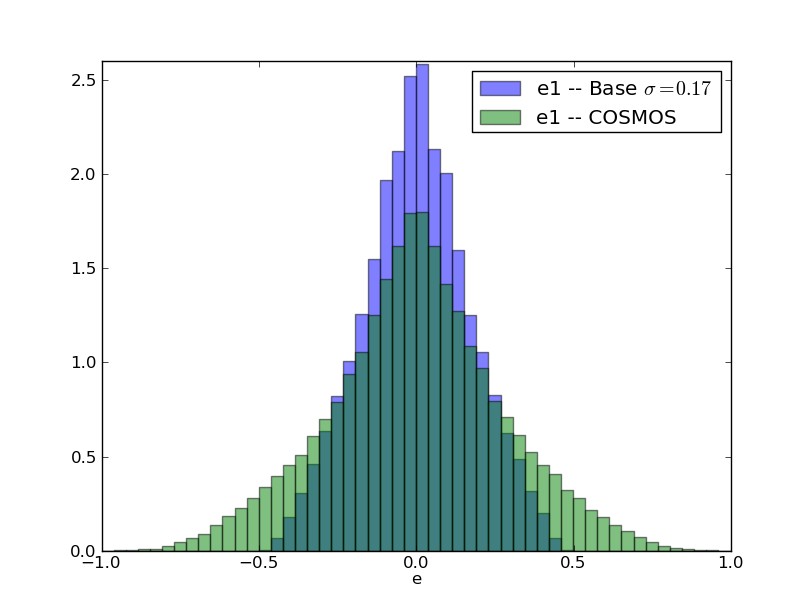
\includegraphics[width=\textwidth]{validation_figures/e1_hist_s_17.png}
              \label{fig:ellip_errbig}
     \end{subfigure}
     \begin{subfigure}[b]{0.3\textwidth}
             \centering
             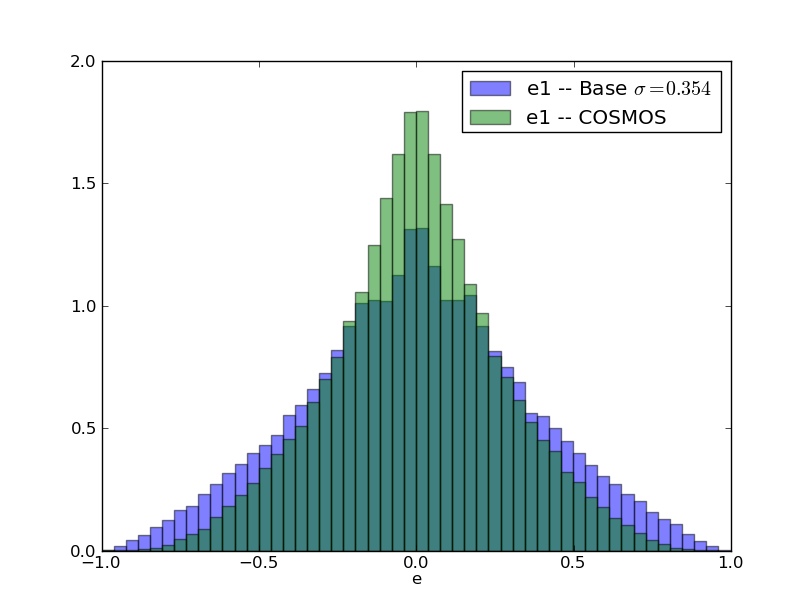
\includegraphics[width=\textwidth]{validation_figures/e1_hist_s_354.png}
            \label{fig:ellip_errbig}
     \end{subfigure}

\caption{Histogram of e1 values for the base catalog and COSMOS sample.  These distributions are for objects with $20.0 < i < 24.5$ to match
the cut made in \citet{chang}.
Same as Figure \ref{fig:ellip1} but for e2.
The base catalog distribution with the width scaled such that the requirement is just missed by predicting an $n_{eff}$ value that is too large.
The base catalog distribution with the width scaled such that the requirement is just missed by predicting an $n_{eff}$ value that is too small.}
\end{figure}

For completeness, we show the redshift distributions for 1 magnitude bins from $i=18$ to $i=24$.  See Figure \ref{fig:nofz18_24}.  As shown in \ref{fig:neffvm}
galaxies with $i > 25$ do not contribute significantly to $n_{eff}$. 

\begin{figure}[th]
\centering
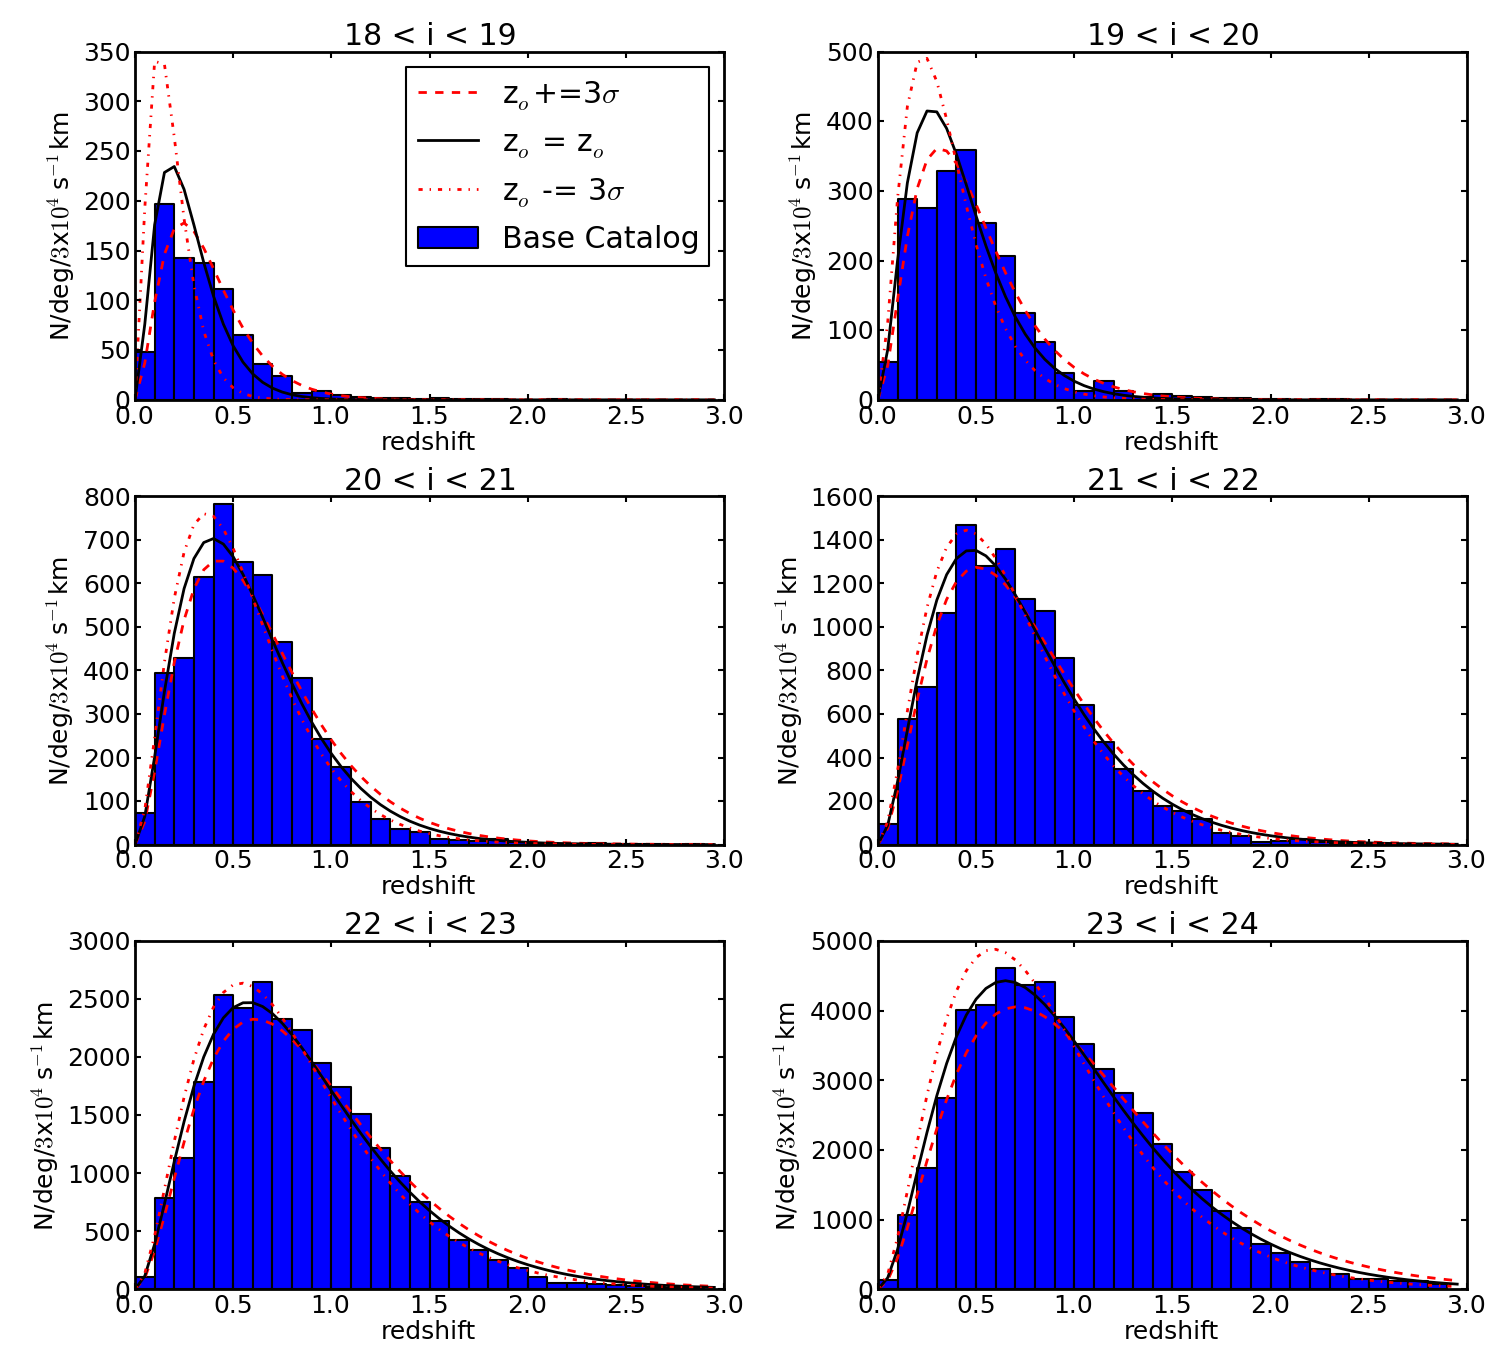
\includegraphics[width=5in]{validation_figures/Nofz_18_24.png}
\caption{The blue histogram in each panel is the measured N(z) for 1 magnitude bins from $18<i<24$.  Over-plotted is the empirical distribution from \citet{coil04} normalized to the area of the measured distribution.  The dashed and dotted red lines show what happens if the governing parameter for the \citet{coil04} distribution, $z_o$, is over
or under predicted by $3\sigma$ respectively.\label{fig:nofz18_24}}
\end{figure}
%\begin{figure}
%\centering
%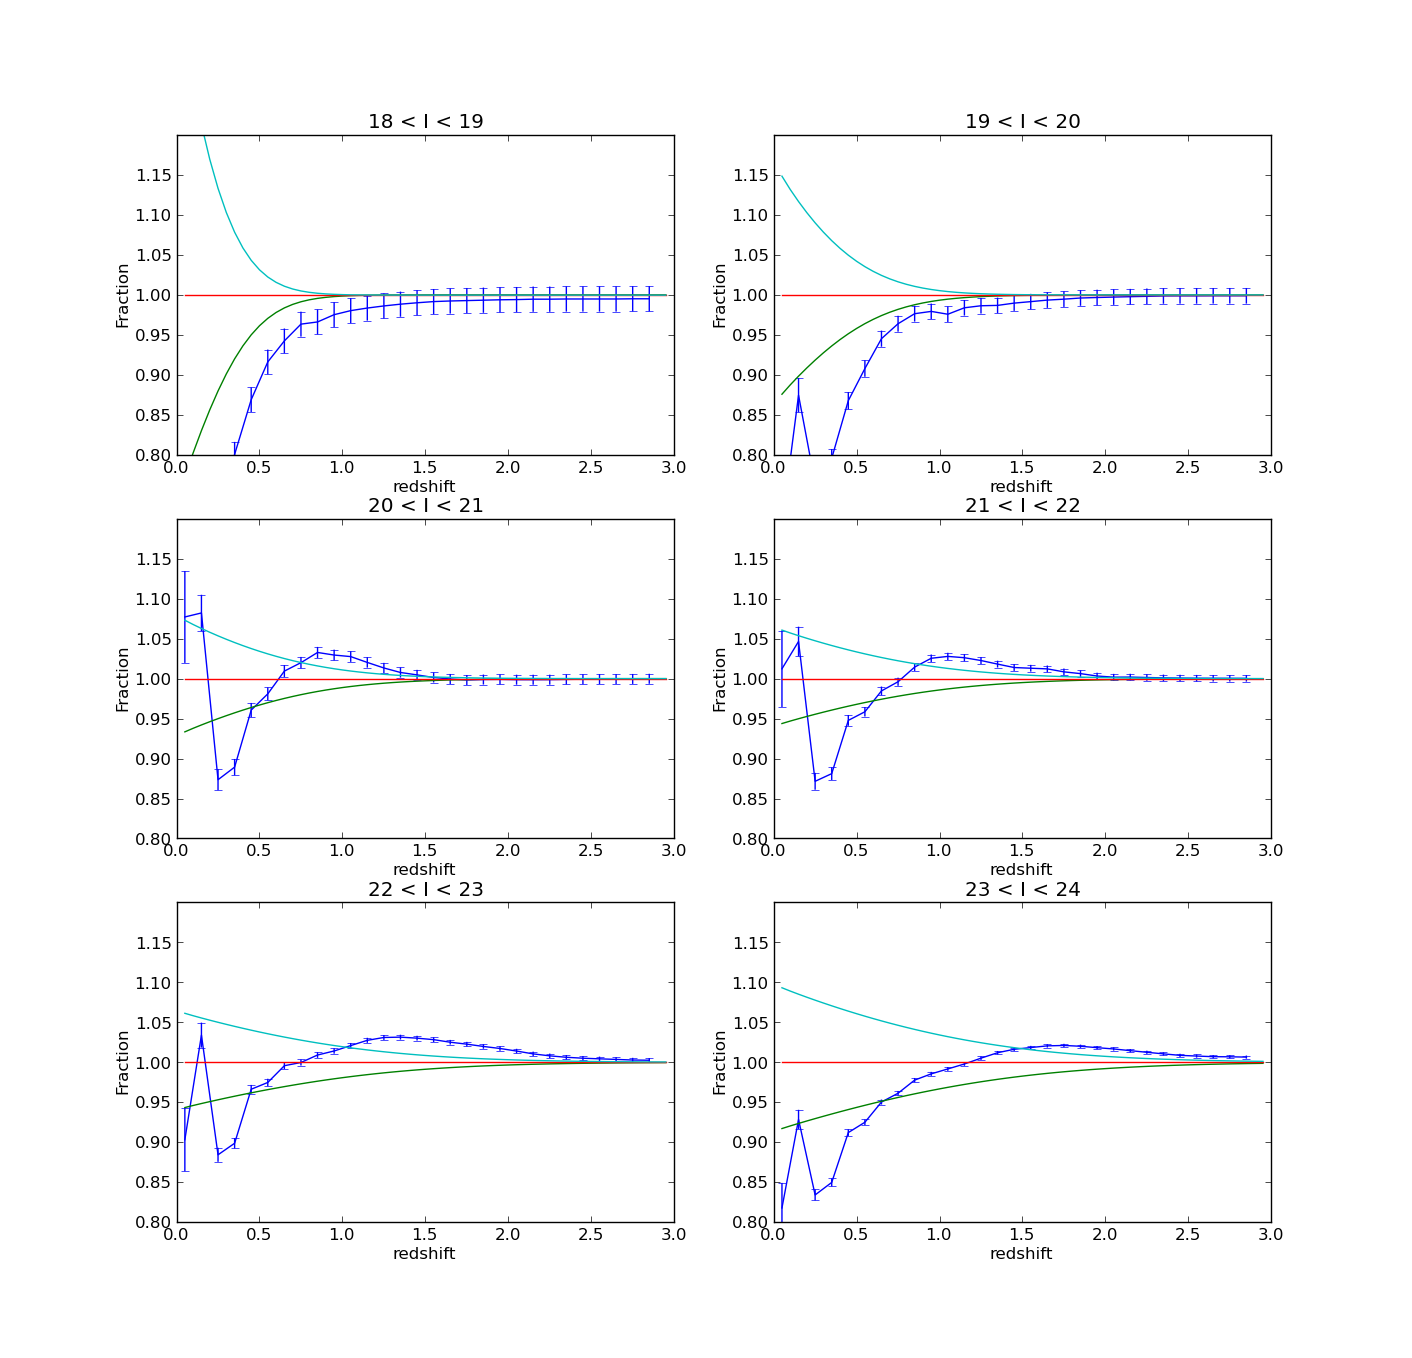
\includegraphics[width=5in]{validation_figures/Nofz_CumulativeFraction_18_24.png}
%\caption{N(z) for 18 to 24 with distribution from \cite{coil}\label{fig:nofz18_24_ratio}}
%\end{figure}
%\begin{figure}
%\centering
%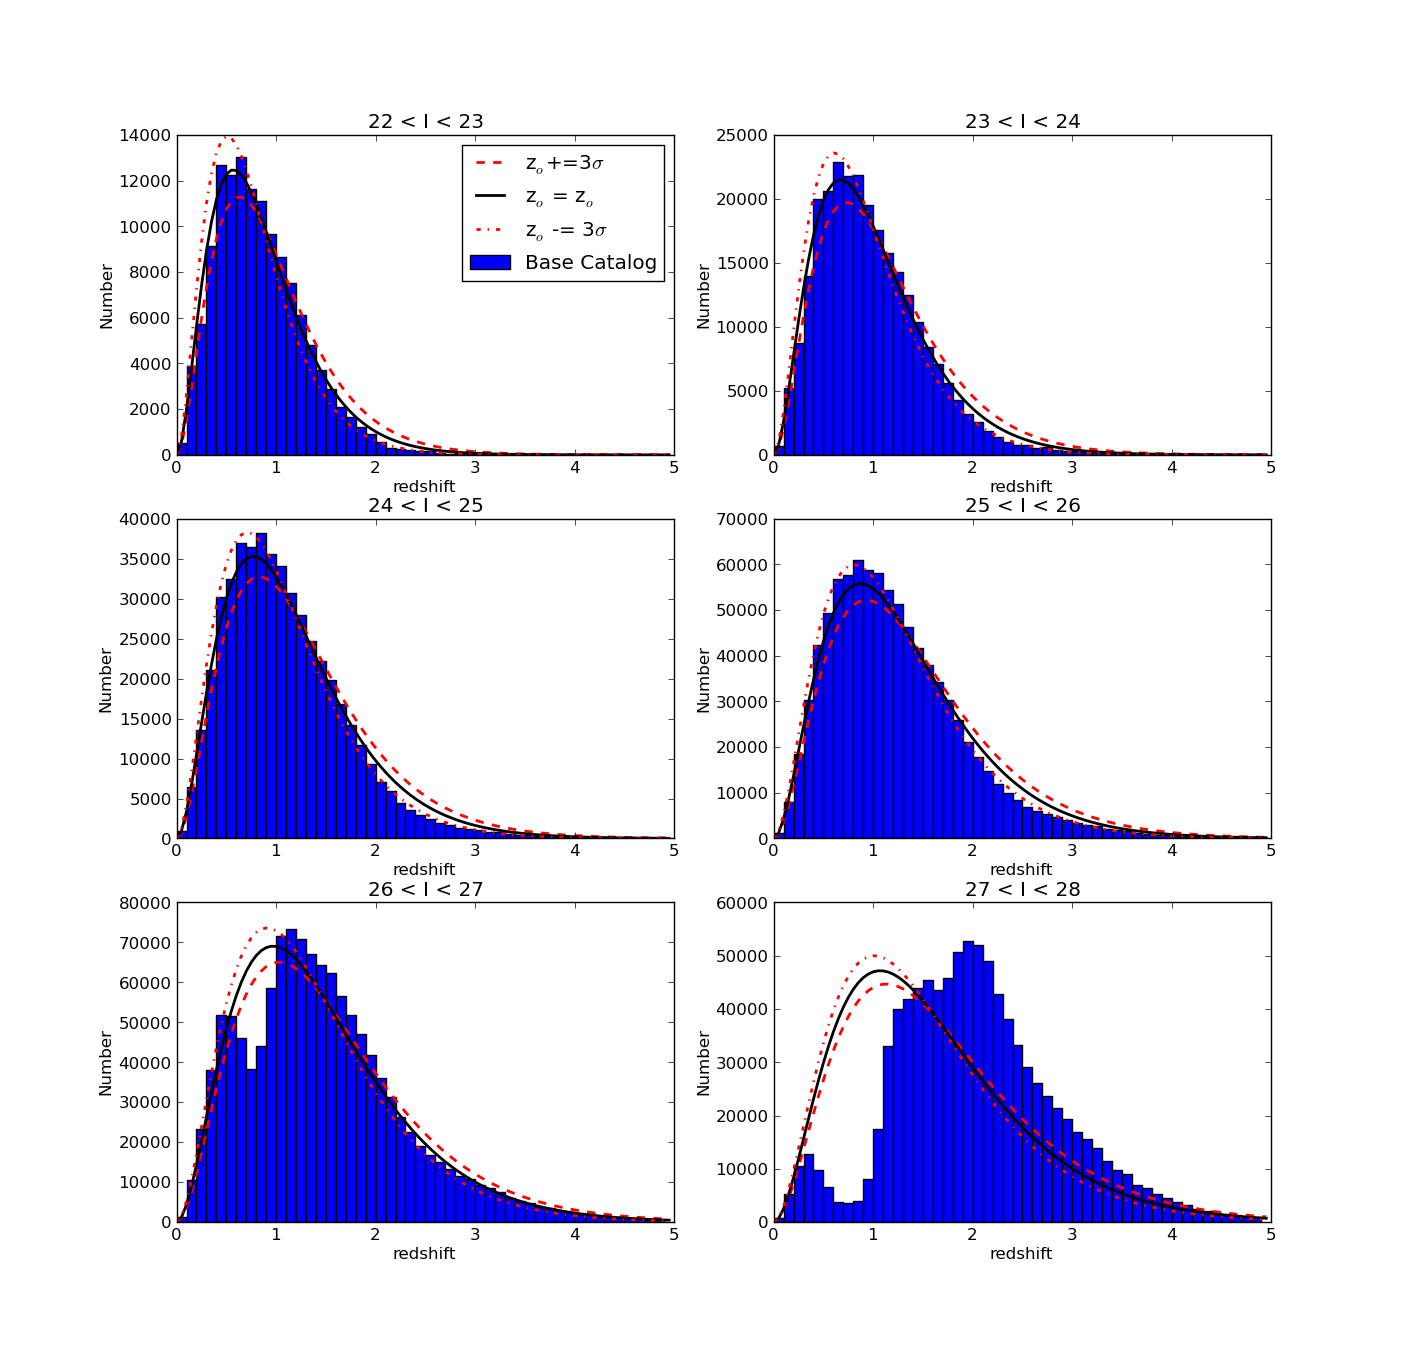
\includegraphics[width=5in]{validation_figures/Nofz_coil_22_28.png}
%\caption{N(z) for 22 to 28 with distribution from \cite{coil}\label{fig:nofz22_28}}
%\end{figure}
%\begin{figure}
%\centering
%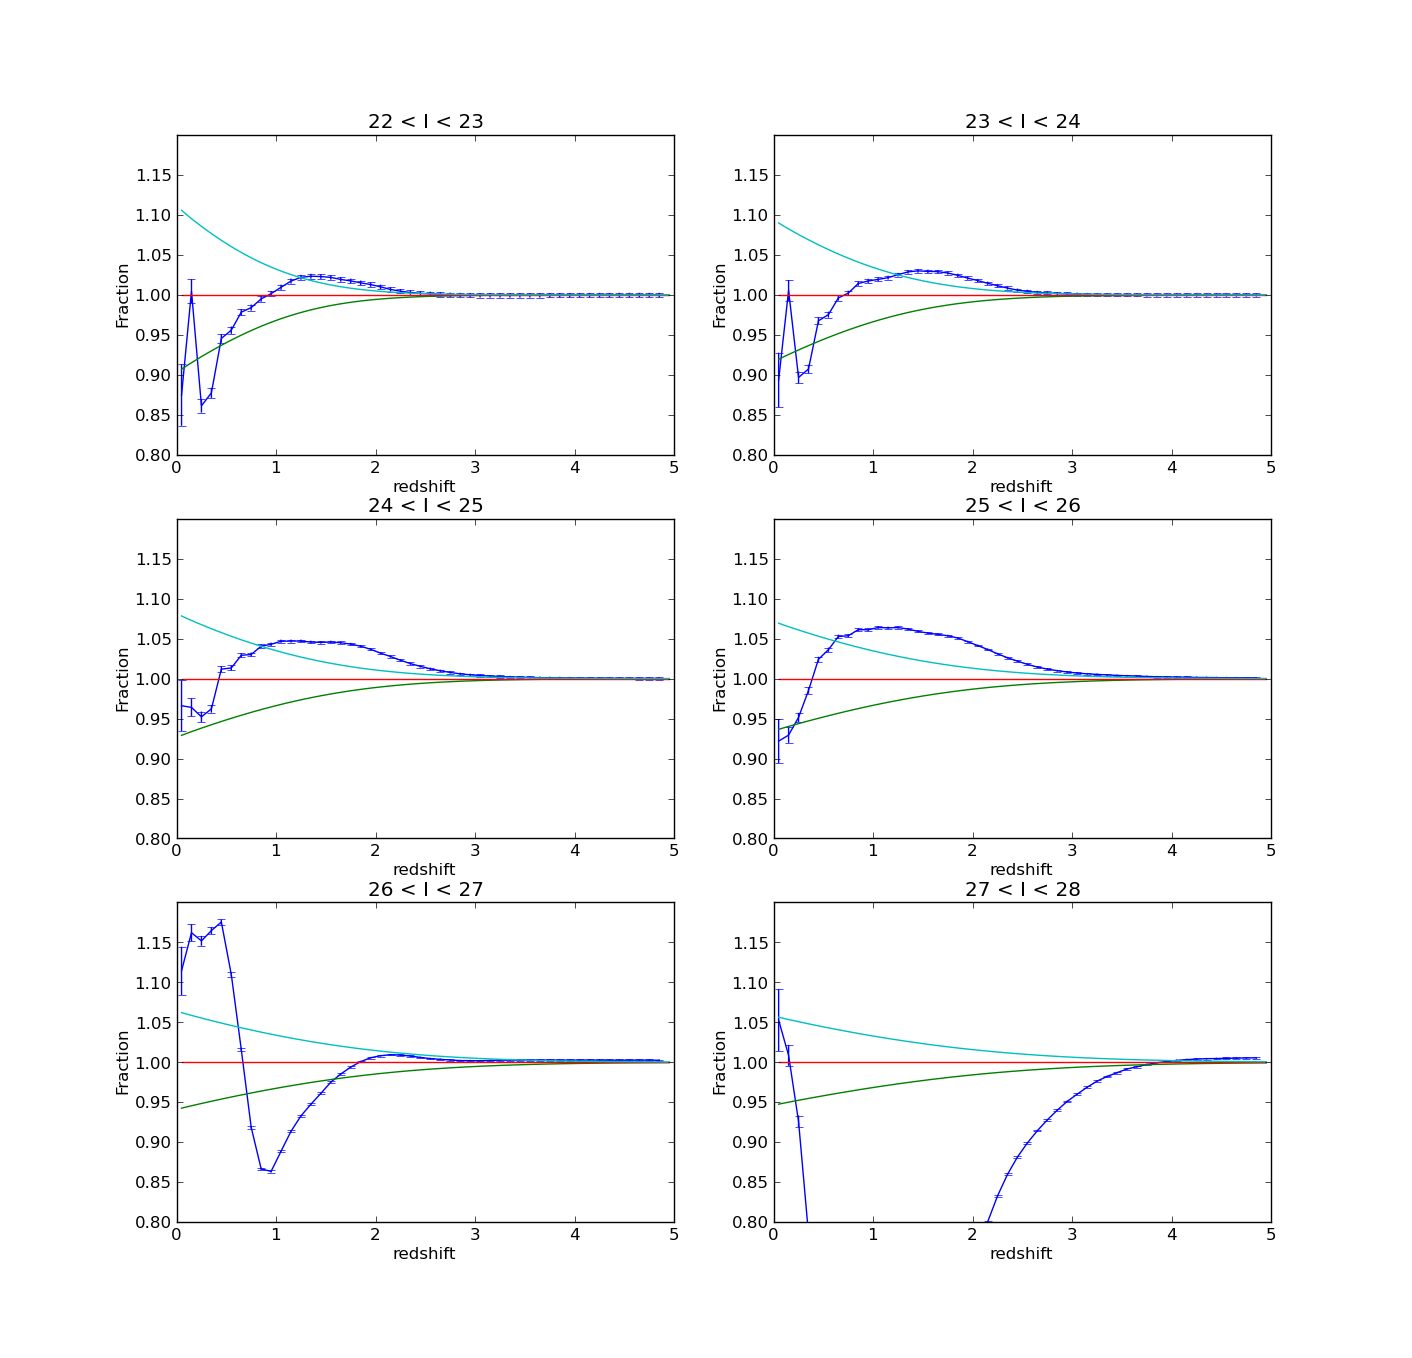
\includegraphics[width=5in]{validation_figures/Nofz_CumulativeFraction_22_28.png}
%\caption{N(z) for 22 to 28 with distribution from \cite{coil}\label{fig:nofz22_28_ratio}}
%\end{figure}
\begin{figure}[H]
\centering
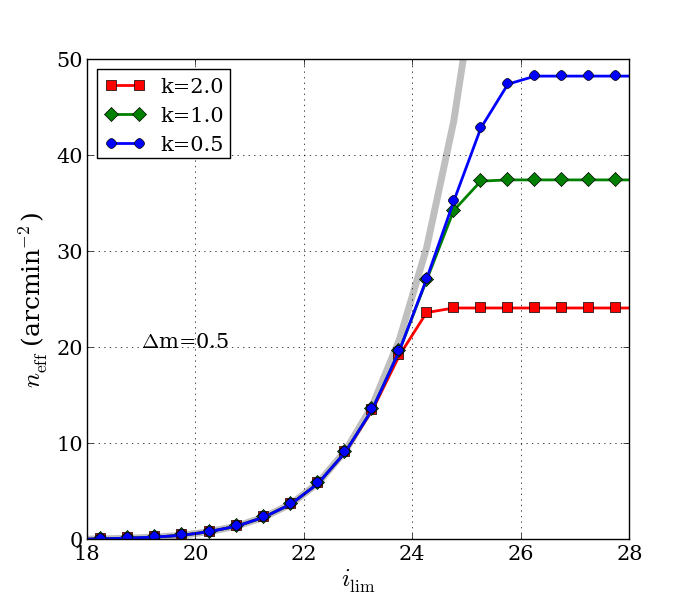
\includegraphics[width=0.5\textwidth]{validation_figures/neff_m_ir.png}
\caption{This shows $n_{eff}$ as a function of i-band limiting magnitude.  Even though the the density of galaxies is going up steeply, the 
size of the galaxies relative to the PSF is falling off quickly enough that galaxies fainter the $i=25$ don't contribute much to $n_{eff}$.\label{fig:neffvm}}
\end{figure}


\subsubsection{Galaxy radius measurements}
There are many definitions of galaxy size: half light radius, first
moment radius, second moment radius, Petrosian radius, Kron radius,
etc.  For the validation of the galaxy size distributions we utilize
data from the COSMOS Advanced Camera for Surveys catalog \citep{cosmos} as it
extends to depths greater than $i=24.5$, is of higher resolution than
ground-based data (i.e.\ with an image quality of $<0.1$ arcsec), and
covers a representative area of the sky (2 deg$^2$). The COSMOS catalog reports both the second moments and the 
half light radius. 

One concern in comparing observed and model radii is that the base
catalog are effectively infinite signal to noise, whereas the
measurements from COSMOS are not.  We, therefore, consider the impact
of the S/N on the derived sizes in order to define the appropriate
measure to use for comparison. We model the effects of signal-to-noise
on the half-light and second moment radii by truncating the Sersic
profiles at a specified radius (i.e.\ reproducing the effect of the
light profile dropping below the noise in the image).  We truncate the
profiles at multiples of the half light radius, $R_{hl}$: $1.33R_{hl},
1.78R_{hl}, 3.16R_{hl}, 10R_{hl}, $and$100R_{hl}$. {\bf XXX what does
  this correspond to in S/N?}


Figures \ref{fig:hl_hist} and \ref{fig:mom_hist} show the effect of
progressively decreasing the signal-to-noise of a light profile.  As
the signal-to-noise decreases the peak and width of the distributions
of half light and second moment radii decrease (see Figure
\ref{fig:mom_hl_line}).  Going from $100R_{hl}$ to $10R_{hl}$ the mean
of the second moment radius distribution decreases by $0.14\%$ and is
half the high signal-to-noise value at $1.78R_{hl}$.  By comparison,
the mean of the half light radius distribution decreases by less than
$1\%$ going from $100R_{hl}$ to $10R_{hl}$ and is $22\%$ of the high
signal-to-noise distribution.  The width of the distributions exhibit
similar behavior with the second moment radius distribution impacted
much more heavily by the reduced signal-to-noise than the half light
radius distribution.  Because of the stability of the half light
radius distribution in the presence of noise, we compare the half
light radius from the Universe model to observed data sets.

\begin{figure}[ht]
\centering
\begin{subfigure}[b]{0.4\textwidth}
  \centering
 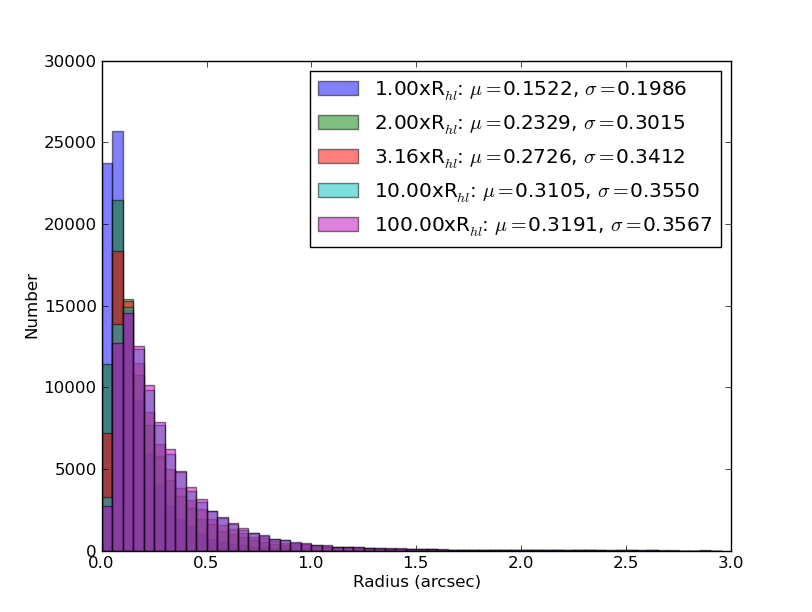
\includegraphics[width=\textwidth]{validation_figures/half_light_hist.png}
  \label{fig:hl_hist}
\end{subfigure}
\begin{subfigure}[b]{0.4\textwidth}
  \centering
  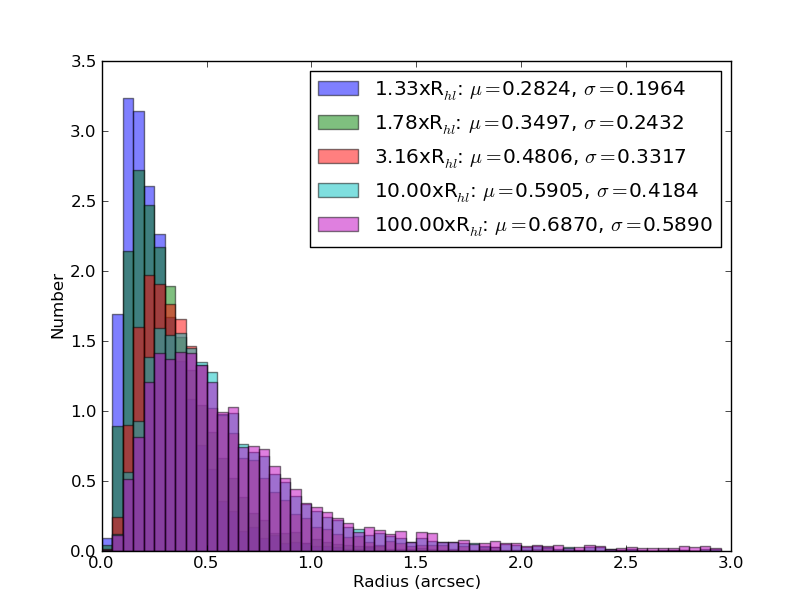
\includegraphics[width=\textwidth]{validation_figures/Second_moment_hist.png}
  \label{fig:mom_hist}
\end{subfigure}
\caption{Modelling the impact of signal-to-noise on measures of
  radii. The truncation for each distribution is listed in the legend
  along with the mean and standard deviation at that value of the
  truncation.  Truncating the Sersi{\'c} at smaller radii approximates
  lower signal-to-noise measurements.  The left panel shows the
  distributions for half light radii and the right panel for second
  moment radii}
\end{figure}


\begin{figure}[ht]
\centering
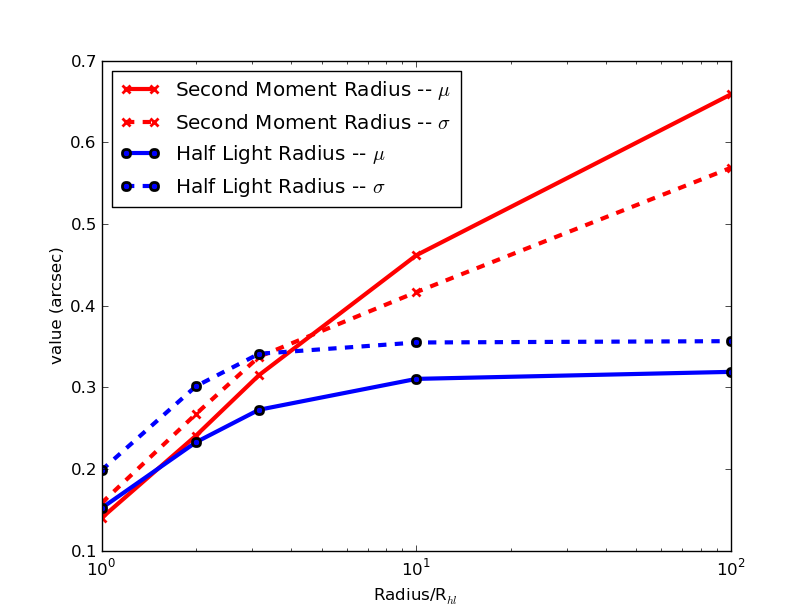
\includegraphics[width=0.5\textwidth]{validation_figures/sec_mom_half_light_mean_sigma.png}
\caption{The mean and standard deviation of the half-light and second
 moment radii as a function of the truncation in the Sersic profile.}
\label{fig:mom_hl_line}
\end{figure}

To evaluate the sensitivity of $n_{eff}$ on size, we model the 
half light distribution as a log normal distribution.  Figure
\ref{fig:ln_fit} shows log-normal fits to the base catalog and COSMOS
data half light radius distributions.  The half light radius
distribution for the base catalog is dominated by the disk components
since there are many more disk only objects than bulge only objects
and the disk components have large half light radius values (relative
to the bulge).  To simulate varying half light radius distributions we
take the bulge distribution from the base catalog and then sample from
a log-normal distribution with varying shape parameters.
{\bf XXX what does this mean?}
\begin{figure}[H]
\centering
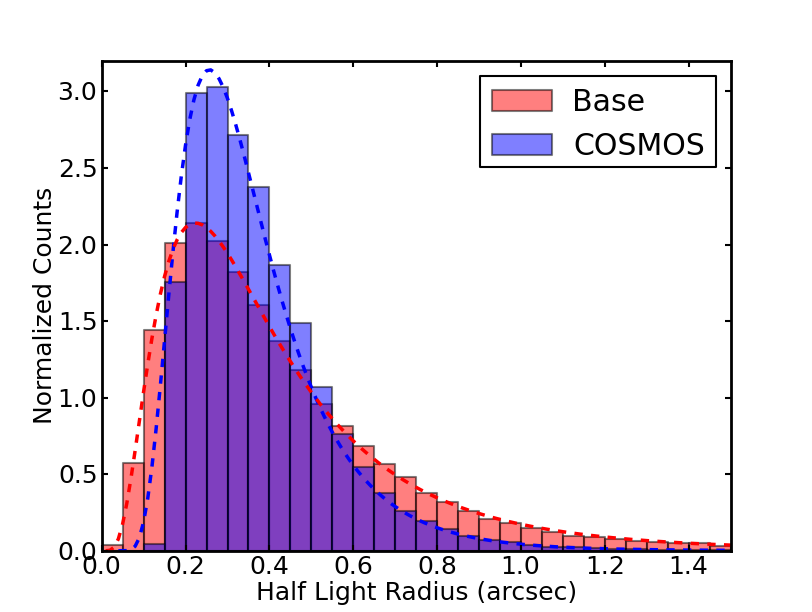
\includegraphics[width=0.5\textwidth]{validation_figures/ln_fit.png}
\caption{{\bf XXX This figure needs to be remade, it was done with
    only objects 20 - 24.5.}\label{fig:ln_fit}, why doesnt the
  lognormal fit why isnt there a discussion of base +psf}
\end{figure}

Figure \ref{fig:size_sens} shows the sensitivity of $n_{eff}$ to the
size distribution.  The x axis is the width of the size distribution
and the y axis the location of the peak of the size distribution. The
contours represent the change in $n_{eff}$ (from its nominal value) as
a function of $x$ and $y$. Over-plotted are points corresponding to
the best fit log normal distributions to the COSMOS data set (black
circle) and the base catalog data set (black square).  The difference
between the COSMOS distribution and the base catalog size distributions
results in a change in $n_{eff}$ of less than 2. 

Combining in quadrature the error in $n_{eff}$ from the shape noise of
the galaxies, the size distributions of the galaxies, and the
signal-to-noise of the observations the total $n_{eff}$ uncertainty is
$XXX$ which is less that the requirement of  $\pm6$ specified for {\it
  Catalogs:  Requirement 3}


\begin{figure}[H]
\centering
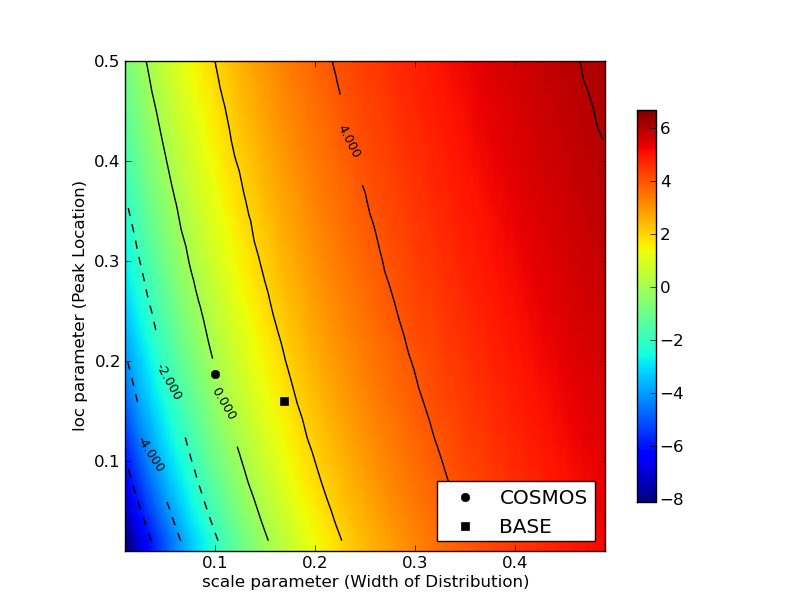
\includegraphics[width=5in]{validation_figures/size_sensitivity.png}
\caption{Sensitivity of the predicted $n_{eff}$ to the shape of the half light radius distribution.  
The surface is normalized to the value of $n_{eff}$ as measured using the half light radius distribution from COSMOS.  The black circle
is the location of the COSMOS data in this plane which by construction falls on the zero contour.  The black square is the prediction of
the measured $n_{eff}$ using the half light radius distribution from the base catalog.\label{fig:size_sens}}
\end{figure}
{\bf XXX why is the bright part not on the delta neff = 0}


\subsection{Catalogs: Requirement 4}

{\it Photometric performance: For the photometric calibration
  simulations the distribution of stellar colors shall encompass the
  colors of white dwarfs through red giant branch stars.  The median
  color distributions of stars must trace the observed color locus for
  these stars to within the 0.02 magnitudes (averaged over intervals
  of 0.3 magnitudes in color). These requirements are defined for
  Galactic latitudes $|b|>30$.}\\


In order to evaluate the sensitivity of the photometric calibration to
the distributions of stars within a focal plane, the Galactic model
must have realistic color distributions.  This includes both the range
of colors spanned by the stellar sources and the fidelity to which
these stars reproduce the observed stellar locus. In Figure
\ref{fig:starcolorspan} we verify that we the stellar catalog meets
the requirement that the colors span the range
\begin{center}
\begin{tabular}{c}
      $ -0.2 < u-g <        2.7 $\\
       $  -0.4  <  g-r <       1.7 $\\
        $ -0.3   <  r-i <    2.3 $\\
        $  -0.25 < i-z <       1.2 $\\ 
        $  -0.2 <  z-y   <    0.8 $
\end{tabular}
\end{center}
For each color ($u-g$, $g-r$, $r-i$,
$i-z$, and $z-y$) we plot the normalized histogram for the main
sequence and red giant branch (RGB) stars (forward hatching) and the
white dwarf (backward hatching).  Together the two distributions span
the required range as shown by the dashed vertical lines in each
panel.
\begin{figure}[H]
\centering
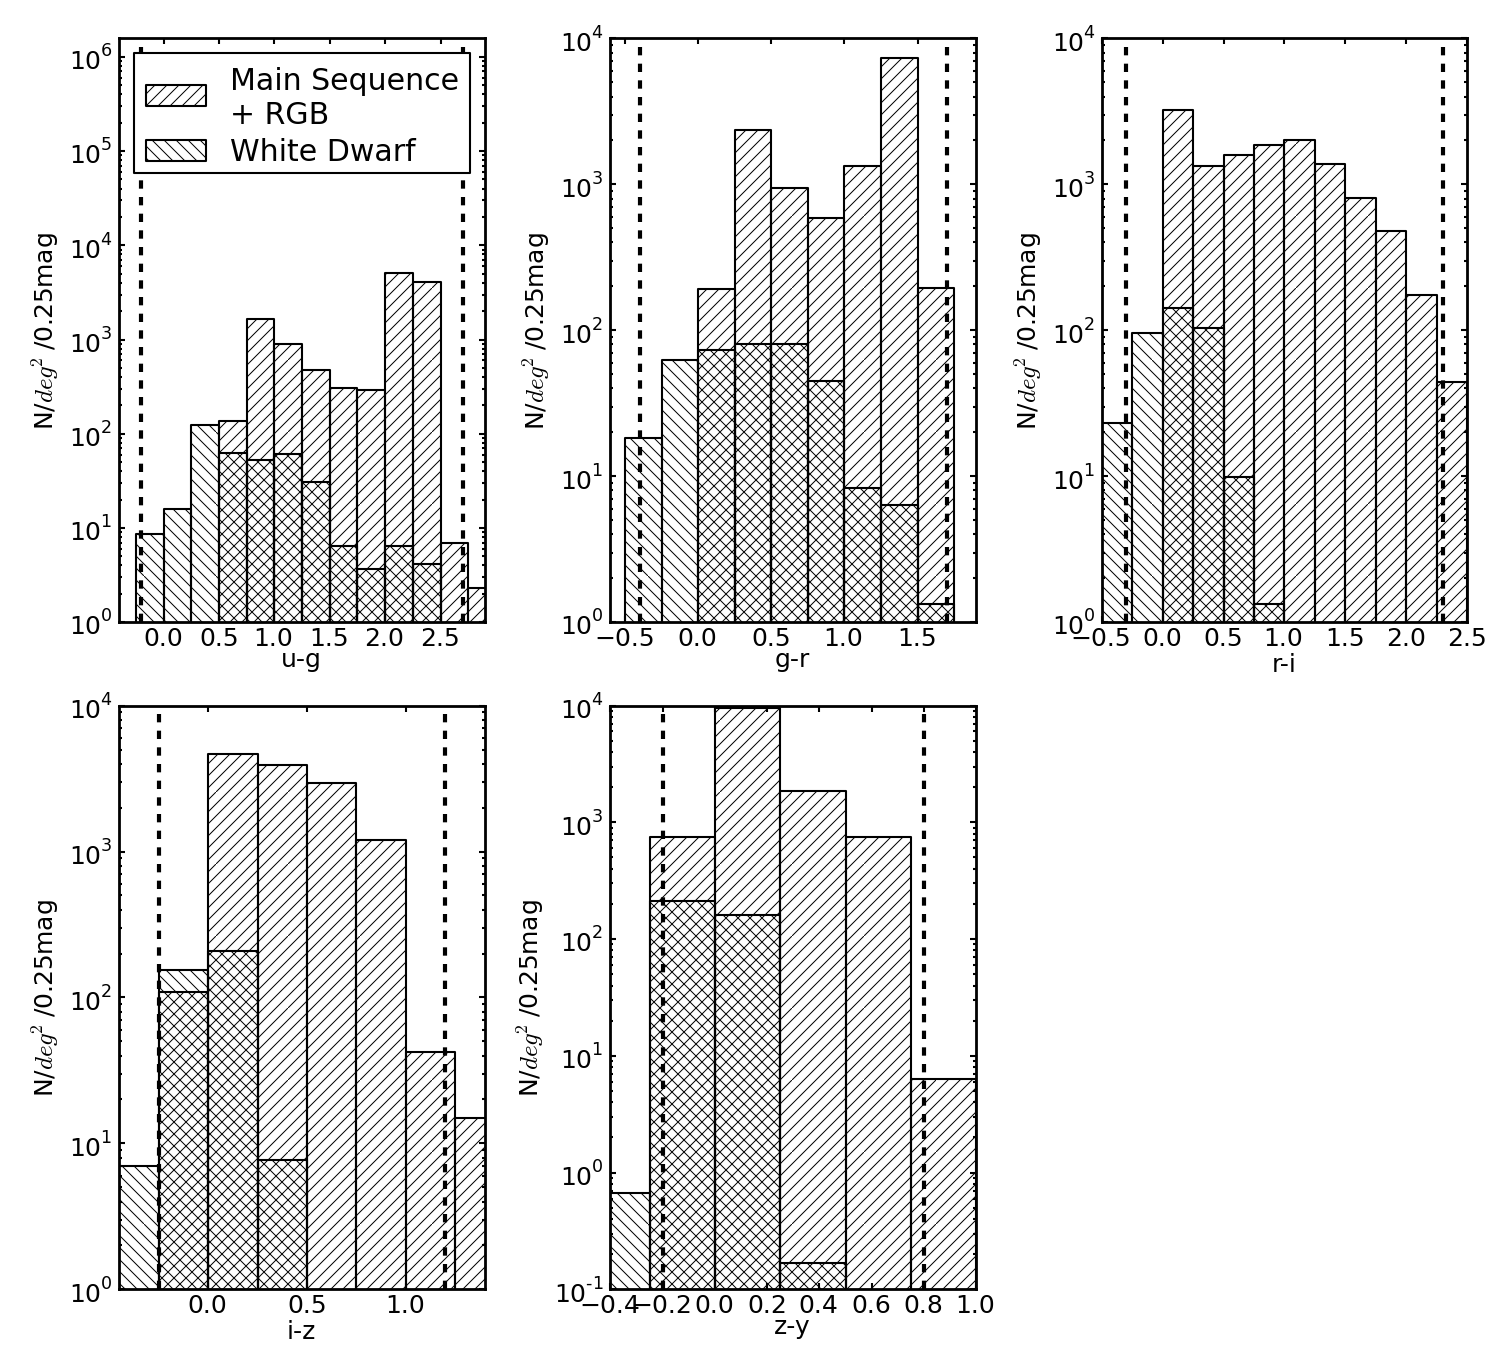
\includegraphics[width=5in]{validation_figures/star_lsst_color_hist.png}
\caption{Normalized counts of main sequence, red giant branch and white dwarf stars as a function of color.  Heavy dashed lines show the requirements given in the requirements document.\label{fig:starcolorspan}}
\end{figure}

To verify the veracity of the main sequence stellar locus, we use the
principal colors of the stellar locus as described by \citet{helmi02}, and 
fit for in the SDSS photometric system by \citet{ivezic04}.
We use stars selected from the same fields as used in the number counts analysis for all fields with $b<-30$.
In order to avoid complications associated with the difference between the LSST and SDSS photometric systems, we calculate the un-extincted 
magnitudes in the SDSS bandpasses using the best fit spectrum for each star.  We then calculate
the principal colors for each star using the relations in
\citet{ivezic04}, but removing the r-band dependence in $P\prime_{2}$
(the $P\prime_{2}$  correction
in \citet{ivezic04} was used to correct for an empirical effect {\bf
  XXX what effect} that is not present in photometry calculated on idealized spectra with idealized throughput
curves). Figure
\ref{fig:principalcolorshist} shows that the principal colors as calculated from the base catalog are in good agreement with
the location of the stellar locus in the SDSS (zero color).  The base catalog easily meets the requirement of $\pm0.02mag$ deviation
from the stellar locus to single epoch depth in all 4 principal colors: ${\Delta}s=-0.003, {\Delta}w=0.001, {\Delta}x=-0.005, {\Delta}y=-0.013$.  
The increase in scatter in the s band when compared to other colors arises from a metallicity dependence in the color.  Figure \ref{fig:sfeh} shows this 
dependence which is consistent with SDSS observations.

\begin{figure}[ht]
\centering
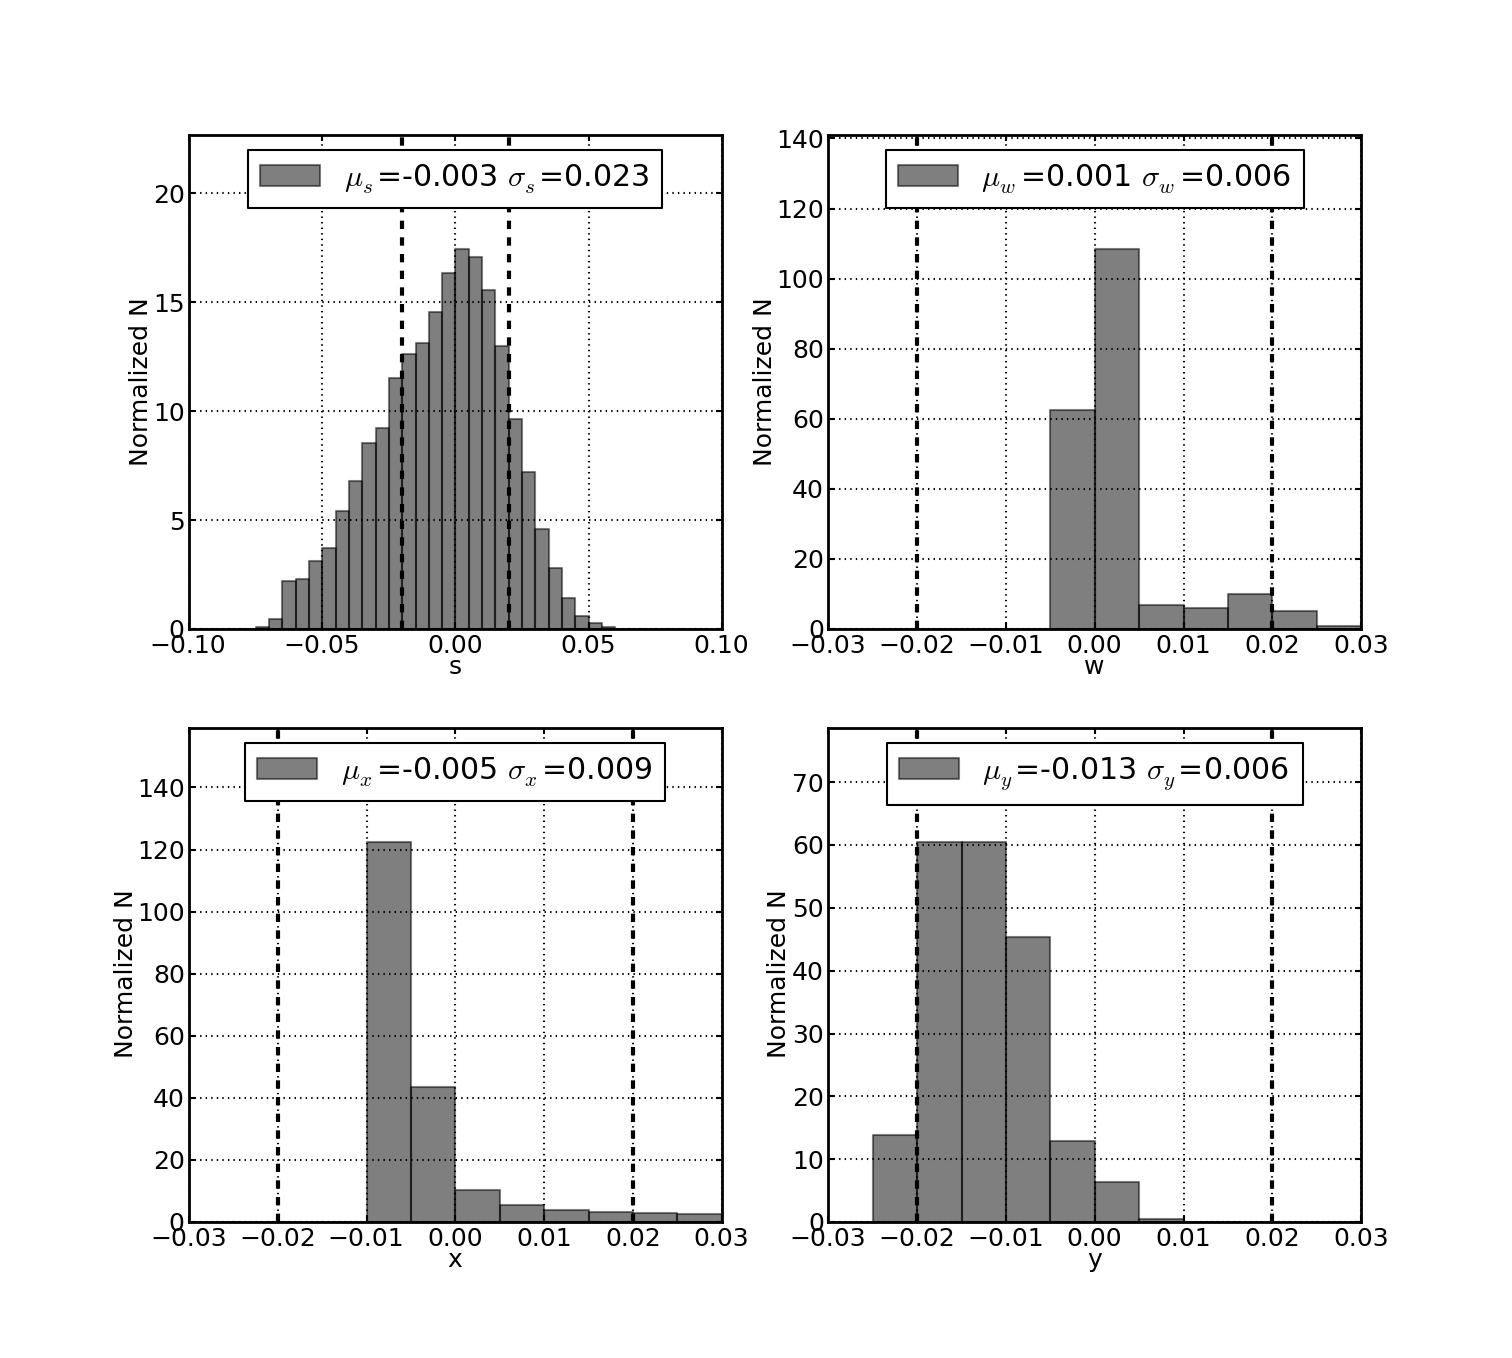
\includegraphics[width=5in]{validation_figures/principal_colors_hist.png}
\caption{Histograms of the principal colors of stars in the base
  catalog compared to SDSS principal colors (zero color in these
  plots) to the stretch single epoch depth of $r < 24.8$. The mean and
  standard deviation for each
histogram are given in the legend in the upper right.\label{fig:principalcolorshist}}
\end{figure}
{\bf XXX plot the requirements}

\begin{figure} [ht]
\centering
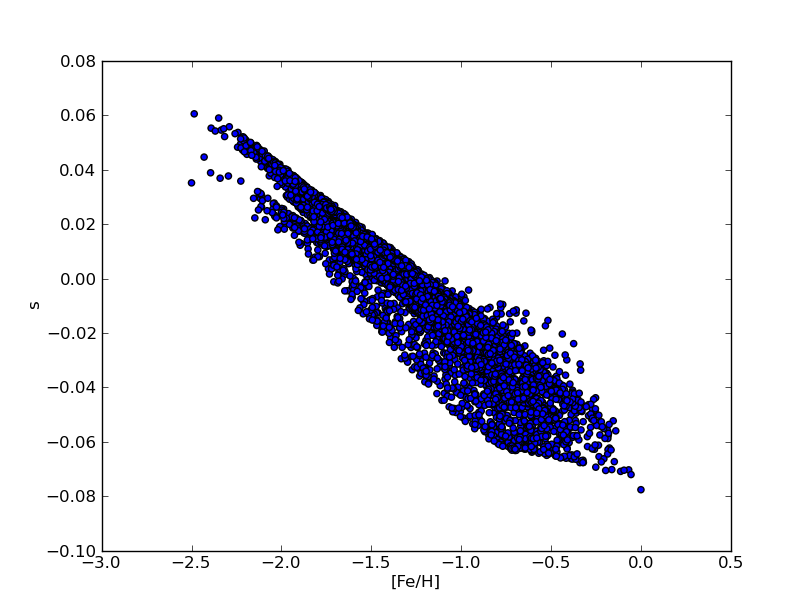
\includegraphics[width=0.5\textwidth]{validation_figures/s_met.png}
\caption{The principal color s as a function of metallicity.\label{fig:sfeh}}
\end{figure}


Figure \ref{fig:principalcolorshist} shows that the requirement of mean deviation from the color locus defined by the four principal colors by less than 
0.02 magnitudes is met in all four bands.

\subsection{Catalogs Requirement 5}

{\it All models for the astrometric transforms applied to the catalogs (including interpolation functions) 
shall have an accuracy better than 1.6 mas}\\

All operations on positions are undertaken using double precision
accuracy. Angular operations are converted to Cartesian coordinates to
provide accuracy at the celestial poles and to minimize the
complications of the coordinate wraparound at the
meridian. Astrometric accuracy of the CatSim simulation framework is
determined from the performance of the Starlink positional astronomy
library (SLALIB; \citealt{wallace}). This software library enables
astrometric transformations and operations with accuracies on the
order of a milliarcsecond or better.  The principal SLALIB routines
used by the CatSim framework are those for precession, nutation,
stellar aberration, rotation of the Earth, diurnal aberration, and
refraction.  As described in \citet{wallace} the definition of ICRS
coordinate system used in SLALIB and its transform to an FK5 (Fifth
Fundamental Catalog - The Basic Fundamental Stars) system has an rms
accuracy that is sub-milliarcsecond. Precession and nutation are based
on the model of \citet{SF2001} and have an rms uncertainty of $<$1
milliarcsecond (with the uncertainty growing at approximately 0.3
milliarcseconds per 1000 years). Aberration and light deflection
corrections are undertaken in an iterative manner with uncertainties
of $<$1 milliarcsecond and the Earth position and velocity corrections
are based on the methods of \citep{stumpff} with a maximum error of
0.3 milliarcseconds. All of these components, added in quadrature,
meet the requirements described in the simulation requirements
document \citet{requirements}.

The largest of the uncertainties in any of the astrometric transforms
are those that arise due to the color dependence of refraction. For a
nominal set of atmospheric conditions (i.e.\ temperature, pressure,
humidity, and lapse rate) the rms astrometric uncertainty is 2.5 mas
over the wavelength range from 0.3 to 1 $\mu$m . This represents a
systematic error on wavelength dependent positions (i.e.\ it is
effectively an error on the parameterization of the model), which is
fit for in deriving an astrometric solution. For the case of CatSim,
while differential chromatic refraction can be applied to catalogs
that are output for science evaluation, the data input to the photon
simulator does not include this effect (i.e.\ it is generated
internally to the photon simulator).

\subsection{Catalogs: Requirement 6}

{\it The system shall be capable of incorporating new astrophysical catalogs without requiring
a redesign of the class-schema framework}\\

The ability to create new catalogs is available within the framework
through the use of user-designed subclasses and class mixins {\bf XXX
  ref}. New types of catalog can be generated by creating a new class using
the InstanceCatalog base class. The columns required in this new catalog are defined
as class attributes. The data for these columns is gathered from the
database directly or using methods defined in the class for the
catalog itself. These data gathering methods can take the form of a {\tt
  get\_[column\_name]} method or in the form of compound columns with
their own {\tt get\_} methods. 

The InstanceCatalog metaclass verifies that all new columns specified
for a new catalog or object reside in the database or can be generated
by user defined methods and functions.  If no method exists and there
is no associated database entry for the column then an error is
raised. Furthermore, this error is raised prior to the query being run
because the instantiation of the class initiates a dry run of the
table output. As a result, the user is protected from errors after the
data is pulled from the database and since all the necessary columns
are determined during the dry run only one single query of the
database is required to pull all necessary data.

An example of the definition of this class structure is provided
below. For this case the user defines the attributes that they wish to
extract form the database (by creating the {\it BasicCatalog} class)
and the operations they wish to apply to these attributes (by creating
the Python Mixin ({\it AstrometryMixin}). A new catalog type is then
created by combining these classes ({\it CustomCatalog}) that
expresses how to output the data. All of the functions and methods
present within the CatSim framework (including photometric, and
astrometric operations) are available to the new class through this
subclassing process (i.e.\ the user simply defines the new operations
that they need).


that extracts a set of user defined columns
from the database (position and id) and transforms the positions into
degrees. Operations on attributes extracted from the database are
defined in a Python Mixin ({\it AstrometryMixin}) and the format of
the output of
the data is defined in a cl 

\begin{verbatim}
class BasicCatalog(InstanceCatalog):
    """Simple catalog with columns directly from the database"""
    catalog_type = 'basic_catalog'
    refIdCol = 'id'
    column_outputs = ['id', 'ra_J2000', 'dec_J2000']
    # transformations specify conversions when moving from the database
    # to the catalog.  In this case, we take RA/DEC in radians and convert
    # to degrees.
    transformations = {"ra_J2000":np.degrees,
                       "dec_J2000":np.degrees}

class AstrometryMixin(object):
    @compound('ra_corrected', 'dec_corrected')
    def get_points_corrected(self):
        ra_J2000 = self.column_by_name('ra_J2000')
        dec_J2000 = self.column_by_name('dec_J2000')
    # ... do the conversions: these are just standins
    ra_corrected = ra_J2000 + 0.001
    dec_corrected = dec_J2000 - 0.001
    return ra_corrected, dec_corrected

class CustomCatalog(BasicCatalog, AstrometryMixin):
    catalog_type = 'custom_catalog'
    refIdCol = 'id'
    column_outputs = ['id', 'redshift', 'points_corrected']
    transformations = {"ra_corrected":np.degrees,
                       "dec_corrected":np.degrees}

# Now to create a catalog, we connect to a database and call write_catalog
db = GalaxyObj()
catalog = CustomCatalog(db)
catalog.write_catalog("out.txt")

# out.txt has the following columns:
# id redshift ra_corrected dec_corrected
\end{verbatim}


\section{Future work}
We expect the requirements of the project to continue to evolve.  Informed by interations with the Systems Engineering team and the Data Management team we have 
identified several areas in which future development will likely take place.  Below we itemize these likely areas of future work.
\begin{itemize}
\item Implement bright stars -- For guiding and wavefront sensing analysis
\item Implementation of extended and morphological images -- Multifit, supernova analysis, galaxy models
\item Reduction of SED data size using PCA -- Parallelization of catalogs generation
\item Add errors to catalogs -- Calibration simulations
\item Add SNe to the catalogs to the framework -- Supernova sensitivity analysis
\item Increase size (area) of galaxy catalogs including cosmological signatures -- Large scale structure
\item Add weak lensing to the catalogs -- Weak lensing
\item Add extended stellar sources, e.g. clusters -- Deblending
\item General variability model -- Alert producton and light curve characterization
\item Further validation of the Milky Way model at low galactic latitudes using Pan-STARRS
\item SNe
\item Proper motion induced by binaries
\item Pan-chromatic variability with spectro-temporal surfaces
\end{itemize}
\bibliographystyle{plainnat}
\bibliography{validation}
\end{document}
